%\documentclass[a4paper,oneside,12pt]{report} % n.pag scritto in basso
\documentclass[a4paper,oneside,11pt]{book}   % Capitolo e n.pag scritti in alto 

\usepackage[utf8]{inputenc} % Tutto il testo e' convertito in TeX encoding, cosi' si indica 
\usepackage{graphicx}  % Per gestire le immagini
\usepackage{scrextend} % Per inserire margini laterali
\usepackage{titling}   % Per fare la title page con immagine

%% TABLES
% Utile per usare H per svuotare la cache dei floating objects come le table
\usepackage{float}     
% Necessario per rappresentare tabelle su più pagine
\usepackage{longtable} 
% Necessario per creare un nuovi tipi di colonna per le tabelle
\usepackage{array}     
\usepackage{tabu}
\usepackage[a4paper, top=3.5cm, bottom=3.5cm, left=2.5cm, right=3cm, heightrounded, bindingoffset=5mm]{geometry}

% Special table columns to center between cells
\newcolumntype{X}[1]{>{\centering\arraybackslash}p{#1}}
\newcolumntype{C}[1]{>{\centering\arraybackslash}m{#1}}
\newcolumntype{P}[1]{>{\arraybackslash}p{#1}}
\newcolumntype{H}[1]{>{\arraybackslash}m{#1}}

% Aggiunge funzionalità alle captions
\usepackage{caption}   
% Distacca le caption dalle table (verticalmente)
\captionsetup[table]{skip=8pt} 
% Default: 6pt - Margine laterale  tra le celle delle tabelle
\setlength{\tabcolsep}{10pt}      
% Default: 1 - Margine verticale tra le celle delle tabelle
\renewcommand{\arraystretch}{1.7} 

% Package for alloy model representation
\usepackage[dvipsnames]{xcolor}
\usepackage{listings}
\usepackage{alloy/style}

% Clickable references
\usepackage{hyperref} 
% Command for two-part captions for tables/pictures
\newcommand{\captionrasd}[2]{\caption{#1}\par\begin{center}\vspace{-.01\textheight}\small#2.\end{center}}

\title{\LARGE{CLup -- Requirements Analysis and \newline Specification Document}}
\author{Vincenzo Riccio, Giancarlo Sorrentino, Emanuele Triuzzi}
\date{December 26th, 2020}
\begin{document}

\begin{titlingpage} 
    \begin{center}
        
\includegraphics[height=0.52\linewidth]{pictures/polimi}\\ % Logo
        \begin{large}
            Software Engineering 2 \\
            A.Y. 2020-2021\\
        \end{large}
        \vspace{4cm} % Spaziatura verticale
        \begin{large} 
            \textbf{\thetitle} \\
        \end{large}
        \vspace{0.7cm}
        \theauthor\\
        \vspace{7.3cm} % Spaziatura verticale
        \thedate
    \end{center}
\end{titlingpage}

\newpage
\begin{table}[H]
    \begin{tabu} to \textwidth { X[0.3,r,p] X[0.7,l,p] }
        \hline
        \textbf{Deliverable:}   & RASD\\
        \textbf{Title:}         & Requirement Analysis and Verification Document \\
        \textbf{Authors:}       & Vincenzo Riccio, Giancarlo Sorrentino, \newline Emanuele Triuzzi \\
        \textbf{Version:}       & 1.1 \\ 
        \textbf{Date:}          & December 26th, 2020 \\
        \textbf{Download page:} & https://github.com/SirGian99/RiccioSorrentinoTriuzzi \\
        \textbf{Copyright:}     & Copyright © 2020, Vincenzo Riccio, Giancarlo Sorrentino, Emanuele Triuzzi -- All rights reserved \\
        \hline
    \end{tabu}
\end{table}

\pagenumbering{roman}
\tableofcontents
\newpage
\pagenumbering{arabic}


\chapter{Introduction}
    
    \section{Purpose}
    CLup aims to provide chains of stores with a reliable solution to the problem of people gathering inside and outside the shops. \par
    To face the problem, the application focuses on its principal causes, which are the management of people inside the store, that often leads to overcrowding, the effectiveness of standard queuing systems and the way people are allowed to visit the stores. Moreover, the system aims to provide a useful tool for store managers in order to help them in administering stores and monitoring their status. In particular, the main goals that CLup aims to achieve, summarized in the table below, are the following: 

    \begin{itemize}
        \item Prevent stores from being overcrowded, in order to avoid indoor gatherings while maximizing their occupancy;
        \item Reduce gatherings of people outside the stores waiting to enter them;
        \item Provide a more efficient way to access stores, reducing the time customers waste while waiting to do it;
        \item Help store managers in monitoring the status of the stores and regulating the influx of people inside them.
    \end{itemize}
    \begin{table}[H]
        \centering
        \begin{tabular}{|>{\bfseries{}}X{0.1\textwidth}|H{0.75\textwidth}|}
            \hline
            \multicolumn{2}{|c|}{\textbf{Goals}} \\
            \hline
            G1 & Prevent stores from being overcrowded while maximizing their occupancy \\
            \hline
            G2 & Reduce gatherings of people outside the stores waiting to enter them          \\
            \hline
            G3 & Reduce the time customers waste while waiting to access the stores       \\
            \hline
            G4 & Help store managers in monitoring the status of the stores and regulating the influx of people inside them \\
            \hline
        \end{tabular}
        \caption{Goals}
        \label{table:goals}
    \end{table}
    
    \section{Scope}
    During the current situation of emergency, it is fundamental to prevent contacts among people. For this reason, governments impose strict rules concerning social distancing, both for indoor and outdoor contexts. \par
    However, crowding management inside stores like supermarkets and grocery shops could be challenging. Currently, stores limit the maximum number of people allowed, and therefore long queues arise: entering a store for a few minutes might even require hours. Moreover, customers who see a crowded store might avoid lining up to save time and prevent contact with others. \par
    CLup fits into this context allowing customers to remotely line up in a queue of a given store and to be notified when they should head toward it. Furthermore, it allows the customer to book a visit to a store on a specific day and time, which grants him priority over the queued customers. \par
    Users can interact with CLup thanks to two distinct interfaces: one is an easy-to-use application designed for the customers, while the other one is an administrative tool that allows store managers to monitor their stores and modify their parameters. \par
    Moreover, CLup also provides physical proxies outside the stores as a fallback option for customers who want to line up but do not have access to the application.
    
    \subsection{World Phenomena}
    The following table illustrates the phenomena that happen in the real world and affect the system, which cannot control or detect them.
    \begin{longtable}[c]{|>{\bfseries{}}c|H{.65\textwidth}|}
        \hline
        \multicolumn{2}{|c|}{\textbf{World phenomena}} \\
        \hline
        WP1 & A person reaches a store \\ \hline
        WP2 & Some people gather in a specific area of a store \\ \hline
        WP3 & People wait in front of a store \\ \hline
        WP4 & A store opens \\ \hline
        WP5 & A store closes \\
        \hline
        \caption{World phenomena}
        \label{table:world_phenomena}
    \end{longtable}
        
    \subsection{Shared Phenomena}
    The following table illustrates the phenomena that happen in the real world and can be observed or managed by the system. The following notation is used:
    \begin{itemize}
        \item \emph{MC} for machine controlled phenomena (observed by the world)
        \item \emph{MO} for machine observed phenomena (controlled by the world)
    \end{itemize}

    \begin{longtable}[c] { |>{\bfseries{}}c|H{0.65\textwidth}|>{\em}X{0.05\textwidth}| }
        \hline
        \multicolumn{3}{|c|}{\textbf{Shared phenomena}} \\
        \hline
        SP1   & A customer requests to join the queue from the application & MO \\ \hline
        SP2   & A customer requests to join the queue using the physical proxy & MO \\ \hline
        SP3   & An alert is sent to the customer when he should reach the store & MC \\ \hline
        SP4   & A customer cannot reach the store in time anymore & MO \\ \hline
        SP5   & A customer is allowed to enter the store & MC \\ \hline
        SP5.1 & A customer enters the store & MO \\ \hline
        SP6   & A customer leaves the store & MO \\ \hline
        SP7   & A customer requests to book a visit to the store & MO \\ \hline
        SP7.1 & A customer specifies the estimated duration of the visit & MO \\ \hline
        SP7.2 & A customer specifies which kind of products wants to buy & MO \\ \hline
        SP7.3 & The system suggests booking alternatives to the customer & MC \\ \hline
        SP7.4 & The system accepts a booking request & MC \\ \hline
        SP7.5 & The system rejects a booking request & MC \\ \hline
        SP8   & The system notifies the customer when specific stores are becoming unavailable & MC \\ \hline
        SP9   & The store manager specifies the maximum occupancy of the store & MO \\ \hline
        SP10  & The store manager specifies the maximum occupancy of the product sections & MO \\ \hline
        SP11  & The manager monitors the status of the store & MO \\
        \hline
        \caption{Shared phenomena}
        \label{table:shared_phenomena}
    \end{longtable}
    
    \section{Definitions, acronyms, abbreviations}
    \begin{longtable}[c] { |>{\bfseries{}}C{0.25\textwidth}|H{0.55\textwidth}| }
        \hline
        \multicolumn{2}{|c|}{\textbf{Definitions, acronyms, abbreviations}} \\
        \hline
        WP\boldmath$x$ & World phenomena number $x$, according to the table of world phenomena \\ \hline
        SP\boldmath$x$ & Shared phenomena number $x$, according to the table of shared phenomena \\ \hline
        CLup & Also known as the system. It is the software to be developed \\ \hline
        Customer application & Also known as application. It is used to access the functions provided by CLup \\ \hline
        Administrative tool & The tool provided to store managers in order to administer stores \\ \hline
        Proxy & The physical fallback option for customers that want to use CLup but cannot use the application. It is placed outside the store it belongs to \\ \hline
        Turn Announcement System & An external system which informs customers about who has been allowed by CLup to enter the store it belongs to\\ \hline
        Access Management System & An external system which regulates physical entrances and exits to the store it belongs to by interacting with CLup \\ \hline
        App-customer & A customer who uses CLup functions through the application \\ \hline
        Proxy-customer & A customer who uses CLup functions through the proxy \\ \hline
        Long-term customer & With respect to a certain store, a customer who already used CLup to visit it \\ \hline
        Current occupancy & Also known as occupancy. It can be referred to the store or one of its sections. It is the number of people inside it \\ \hline
        Maximum occupancy & Refers to the store or one of its sections. It is the maximum number of people allowed to be in that area \\ \hline
        Virtual queue & Also known as access queue or simply queue. It represents the set of customers who lined up through the app or the proxy \\ \hline
        Line up & With respect to a customer and a store, it is the event of joining the queue \\ \hline
        Visit request & A customer’s request to visit a store. It can be either a line-up request or a booking request \\ \hline
        Line-up request & A request made by the customer  to line up for a store \\ \hline
        Booking request & A request made by the customer  to book a visit to a store \\ \hline 
        Visit & The realization of a visit request which takes place when a customer enters the store. After the customer exits the store, we talk about \textit{completed visit}, otherwise it is a \textit{visit in progress} \\ \hline
        Visit token & A unique token bound to a visit request. It allows the Customer to enter and exit the store \\
        \hline
    \caption{Definition, acronyms, abbreviations}
    \label{table:definitions_acronyms_abbreviations}
    \end{longtable} % Controllo warning
    
    \section{Revision history}
    1.0 -- First version of the document (December 23rd, 2020)
    1.1 -- Second version of the document (December 26th, 2020). Changes on the functional requirements table: one of the functions of the application already described in the document was not listed in the functional requirement table.
    
    \section{Reference documents}
    \begin{itemize}
        \item IEEE standard for Software Requirements Specifications, IEEE 29148--2018;
        \item R\&DD Assignment A.Y. 2020--2021;
        \item Teaching material provided by professors Matteo Rossi and Elisabetta Di Nitto.
    \end{itemize}

    \section{Document structure}
    The reference structure used for the document is the one suggested by professor Matteo Rossi of Politecnico of Milan. It is derived from the IEEE standard, which is used as a reference document (IEEE standard for Software Requirements Specifications, IEEE 29148--2018).
    
    \subsubsection{Chapter 1} 
    Chapter 1 is an introduction to the software to be designed and developed and to the problem that it addresses. It presents the goals that should be achieved and an analysis of the context in which the system will be placed.
    \subsubsection{Chapter 2} 
    Chapter 2 is a more detailed description of the system to be realized, focused especially on a more detailed description of the context, e.g. presenting scenarios and the actors involved, on the product functions and on its requirements. Furthermore, it contains explicit constraints, dependencies and domain assumptions.
    \subsubsection{Chapter 3} Chapter 3 includes specific requirements, with a level of detail sufficient to enable designers to design a system to satisfy those requirements, and testers to test that the system satisfies those requirements. It includes the description of all the functional and nonfunctional requirements, together with the description of the external interfaces, of the use cases and of possible design constraints.
    \subsubsection{Chapter 4} 
    Chapter 4 is a formal analysis of the system using the Alloy model, showing also an instance obtained running the model.
    \subsubsection{Chapter 5}
    Last chapter contains a report on the effort spent by all the members of the group while writing the current document.
    \subsubsection{Chapter 6}
    Last chapter contains references to the tools used during the writing of the current document.


\chapter{Overall description}
    \section{Product perspective}
    \subsection{UML Class Diagram Description}
    The provided UML Class Diagram is intended to provide a high-level model of the reality in which CLup is collocated. The following description aims to better highlight the main characteristics of the model. \par
    CLup manages stores of different chains or autonomous ones. In particular each store, which is composed of different product sections, is associated with its managers and with the chain it belongs to, if there is one. A store is also characterized by its name, its address, its maximum occupancy, its working hours and its product sections, which are parameters specified by store managers. Moreover, other significant attributes inferred by the system are the store current occupancy and the average time customers spend inside it. Each product section is identified by its name and is characterized by a current occupancy and by a maximum occupancy. \par
    Customers can visit the store by making a visit request, and are divided into app-customers and proxy customers. More precisely, a customer is identified as a “different” proxy customer every time he makes a line-up request through the proxy. Indeed, since the proxy is meant to be an easy-to-use fallback option, it is not intended to be able to identify customers. \par
    A visit request is made for the desired store and has different attributes, such as the number of people willing to visit the store and the token that will allow them to visit it. CLup provides two kinds of visit requests: line-up requests and booking requests. \par
    Each store maintains a queue of line-up requests, characterized by its length and its estimated disposal time, and holds booking requests made by app-customers. \par
    Booking requests are characterized by attributes such as the date and time requested by the customer and the expected duration of the visit. Moreover, each booking request can also be associated with the store product sections that the app-customer has specified while placing the booking. \par
    The realization of a visit request is represented by a visit, whose starting time represents the time when the customer who made the request entered the store. This means that a line-up request in the queue of the store it refers to is never associated with a visit and, vice versa, a line-up request which is not in the queue is always associated with a visit. When the customer exits the store, the same visit is considered completed. \par
    Further details on the behaviour of the system are specified in the following sections of the document.

    \subsection{UML Class Diagram} 
    \begin{figure}[H]
        \centering
        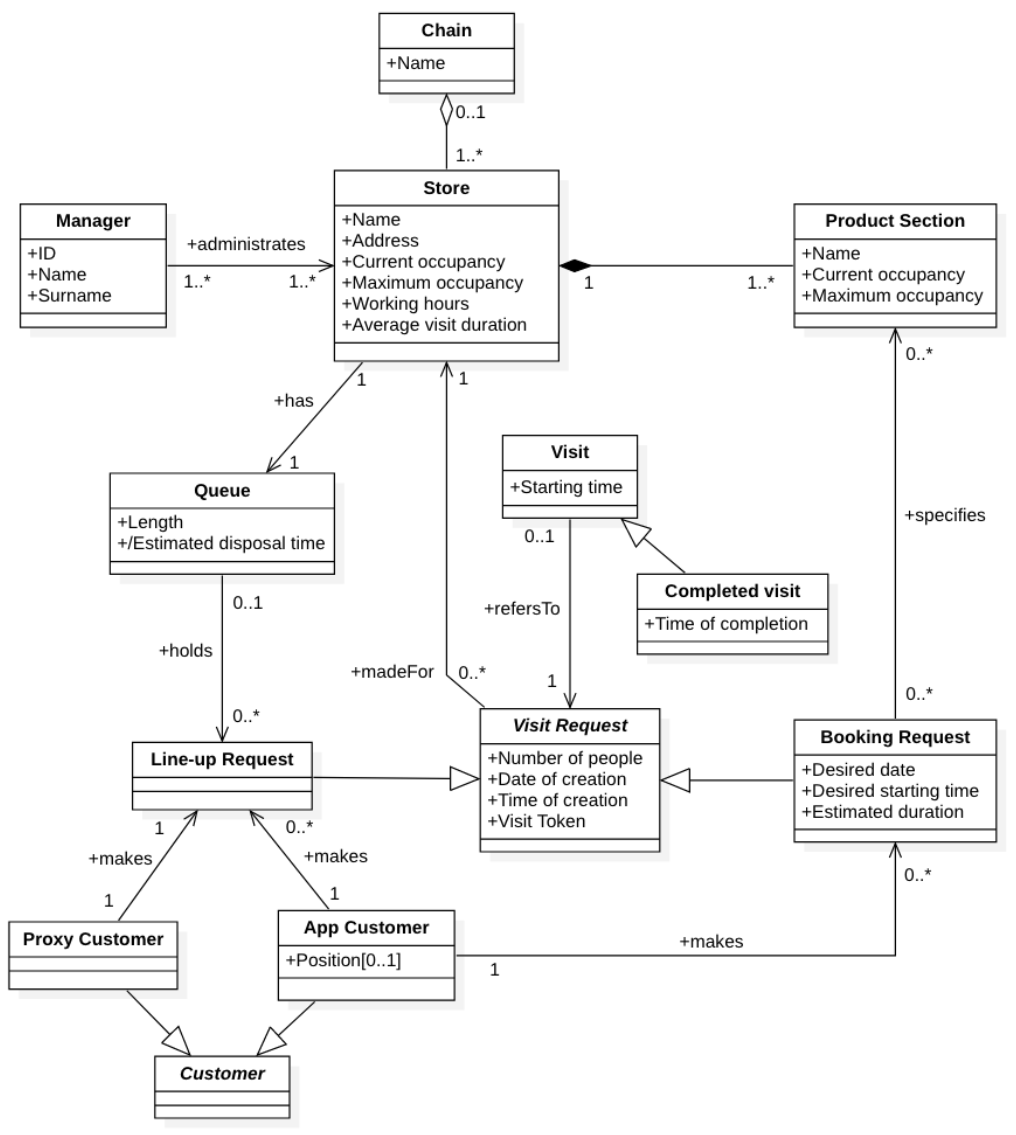
\includegraphics[width=\textwidth, height=\textheight, keepaspectratio]{pictures/uml_class_diagram}
        \caption{UML Class Diagram}
        \label{figure:uml}
    \end{figure}
    \newpage
    \subsection{State charts}
    The following state charts are meant to better explain the status of some classes in the UML class diagram.
    \begin{figure}[H]
        \centering
        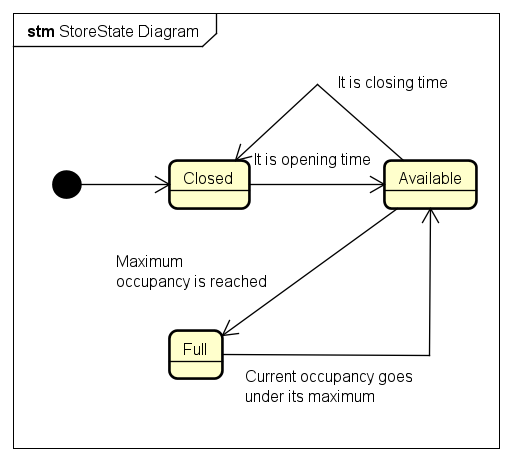
\includegraphics[width=.6\textwidth, keepaspectratio]{pictures/state_diagrams/store}
        \captionrasd{State chart 1 -- ``Store''}{The state chart of the store}
        \label{figure:state_chart_1_store}
    \end{figure}
    \begin{figure}[H]
        \centering
        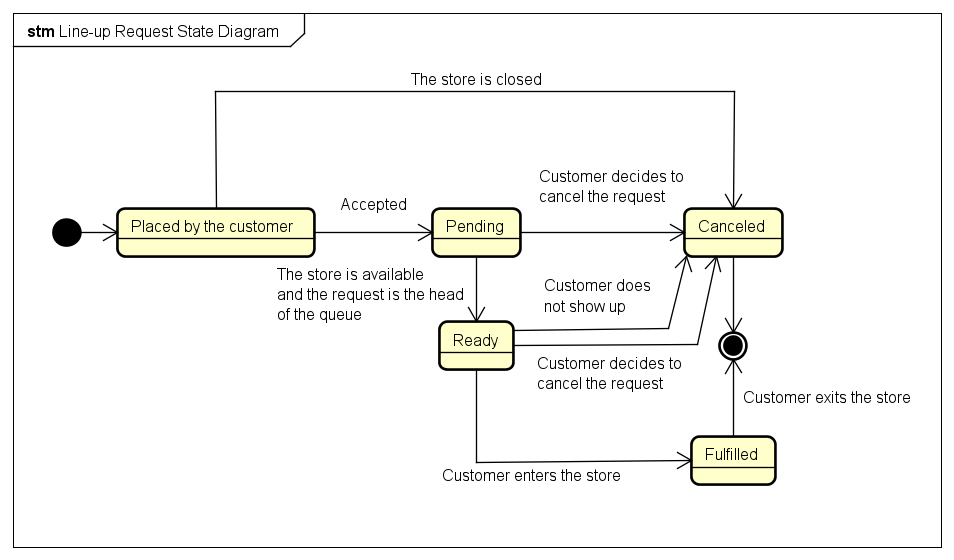
\includegraphics[width=.85\textwidth, keepaspectratio]{pictures/state_diagrams/line-up_request}
        \captionrasd{State chart 2 -- ``Line-up request''}{The state chart of a line-up request}
        \label{figure:state_chart_2_lineup_request}
    \end{figure}
    \begin{figure}[H]
        \centering
        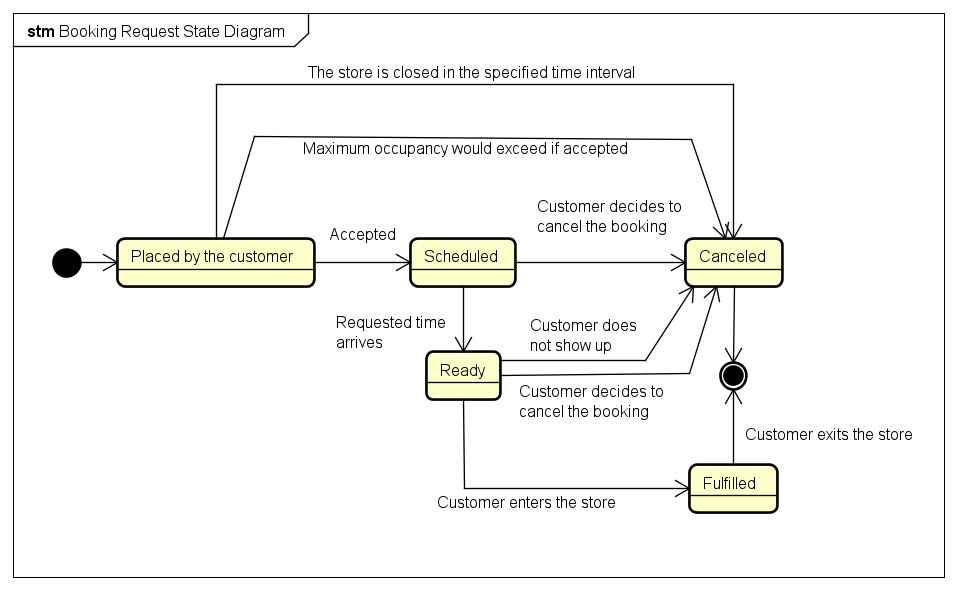
\includegraphics[width=.85\textwidth, keepaspectratio]{pictures/state_diagrams/booking_request}
        \captionrasd{State chart 3 -- ``Booking request''}{The state chart of a booking request}
        \label{figure:state_chart_3_booking_request}
    \end{figure}
    \subsection{Scenarios}
        \subsubsection{Remotely line up for a store}
        Alice is at home and wants to do some grocery shopping at the store at the end of the street. She opens CLup and checks the store’s current queue and the estimated time required to enter. She decides to get in line and starts doing something else. After some time, she receives a notification that suggests her to start heading the store. Thus, she reaches the store. Once there, she opens the app and notices that it is her turn,  so she retrieves the visit token in the app in order to get access to the store. When she is done with her shopping and payment, she opens the app in order to exit the store.
        \subsubsection{Line up for a store using the proxy}
        Bob is a 70-year-old man who is not so keen on using a smartphone, so he has not got any. He has to buy something at the minimarket near his house. He uses the proxy located outside the store to line up and to receive a visit token, and then waits along the street waiting for his turn to come. When it is his turn, he is informed by the Turn Announcement System of the store and enters it by showing the visit token to the Access Management System.  When he is done with his shopping and payment, he uses the visit token in order to exit the store.
        \subsubsection{Booking a visit to a store}
        Chuck is at work and he wants to do some shopping before coming back home. Since there are often many people in line to enter the store he wants to go to, he opens the CLup application and books a visit to the store for a specific time interval. Before reaching the store he must pick up his son from school, so he specifies that two people will visit it. When the time arrives, they have priority over the people in the queue. Since it is their turn, Chuck opens the app in order to get access to the store. After the payment, he opens the app in order to exit the store.
        \subsubsection{Active suggestions for long-term customers}
        Isaac wants to book a visit for Saturday at noon at his local shop. Since he is a long term customer of that chain of stores, CLup provides him with an estimated duration of his visit, based on data about his previous visits. However, the system also informs him that, for the selected time interval, the store is often crowded, and so suggests to him different alternatives. Sadly, George can only do shopping in the indicated one, so he places his booking anyway.
        \subsubsection{Booking alternatives are suggested}
        Emanuele lives near a store in “via Rubattino” and wants to do some grocery shopping next Saturday morning at 11 a.m. However, that store is already at its maximum occupancy in the selected time interval due to previous bookings by other users. So, when Emanuele tries to place a booking request, the system provides him with two alternatives: the first one is to book a visit on the same day at 6 p.m., when the store, according to bookings and statistics, will be less crowded; the second one is to book a visit for the same time interval in another store of the same chain, which has not reached its maximum occupancy yet. Emanuele chooses an option and fulfils his need. 
        \subsubsection{There is always a way out}
        Giancarlo is a customer who is currently visiting a store. While in the store, he notices that his phone ran out of battery. After he is done with his shopping, he asks for the help of a store manager, who manually allows him to exit the shop. The occupancy of the shop is then automatically updated.
        \subsubsection{Forgetting about the visit}
        Vincenzo is a forgetful man. When his turn comes, he is not outside the store. CLup detects Vincenzo is not showing up and allows another customer to enter.
    
    \newpage
    \section{Product Functions}
    CLup is intended to manage different chains of stores and autonomous stores. Each store has at least one manager who can specify, through the administrative tool, different parameters: the name, the address, the working hours, the store maximum occupancy and its product sections (and their relative maximum occupancies). Furthermore, managers can also use the tool to monitor the status of the shop, which includes:
    \begin{itemize}
        \item the number of people inside;
        \item the visits which are actually in progress;
        \item the average duration of a visit;
        \item the actual length and estimated disposal time of the queue;
        \item all the future booking requests.
    \end{itemize}
    CLup regulates the influx of people in a store to prevent it from being overcrowded. To do so, the system  provides a way to authorize the entrances to each shop with respect to the number of people inside it. \par
    The system uses unique visit tokens to authorize each customer to enter and exit a store. In fact, in order to visit the store, customers must provide their visit token to the Access Management System of the store, which will let them enter and exit the store by communicating with CLup. If the customer uses the application, the visit token will be available in the application itself. Instead, each time a customer uses the proxy of a given store, a visit token is physically provided by the proxy itself. All the accesses are granted by CLup with respect to the store maximum occupancy. \par
    In order to reduce the possibility of queues forming outside the stores it manages, CLup provides the possibility to remotely line up in the queue of the desired store. A customer can join the queue either by using the application offered by CLup or by means of the proxy placed outside the store. \par
    Furthermore, CLup alerts app-customers when they need to reach the store they requested a visit for, taking into account the time they need to get to the shop from their current position with respect to the time at which they will be authorized to enter it. Eventually, the system informs customers when they are allowed to enter the store through the Turn Announcement System and, for app-customers, also through the application. \par
    An app-customer can also use the application to book a visit to a store. Doing so, he has to specify when he wants to reach it, the expected duration of the visit and, if he wants, which kind of products he intends to buy. In the case of a long-term customer, the duration of the visit can also be estimated by CLup taking into account his previous visits to the selected store. \par
    All these data are used by the system to manage who can enter each store in a specific time interval. \par
    When a booking is placed, the system can also decide to reject it if, across the specified time interval, the bookings placed by other customers already maximize the occupancy of the selected store. The system also tries to balance the number of customers across all the working hours of the store. In both cases, it suggests alternative time intervals or alternative stores of the same chain when a customer is booking a visit. \par
    CLup is able to manage the case in which, for any reason, a customer does not show up while he is allowed to enter the store he requested a visit for, while other people are waiting to enter it. Moreover, app-customers can always cancel their visit requests (both line-up and booking requests), if needed. \par
    App-customers can choose to be notified about the availability of specified stores. Indeed, a customer can specify one or more recurrent time intervals in which he is interested in visiting those stores. These intervals can also be inferred by the system based on the customer’s attitudes. The system will notify him if, during one of those time intervals, the store of interest is reaching its maximum occupancy. Doing so, the customer can take the opportunity to visit it by booking or lining up. \par
    CLup monitors customer attitudes also to estimate the average visit duration of each store.


    \section{User characteristics}
    \subsubsection{Store manager}
    The store manager administers his stores by checking their status and modifying their parameters, such as the working hours and maximum occupancy. He also specifies the different product sections that compose the store and their relative maximum occupancies. He can also keep track of the real-time store occupancy, and might let people in and out of the store, if needed.
    \subsubsection{Customer}
    The customer uses CLup in order to visit a store of a given chain. To do so, he can either line up in the CLup queue by means of the application or the proxy, or also book a visit through the application. 
    \subsubsection{Access Management System}
    The Access Management System is the system which regulates physical entrances and exits to the store it belongs to. It recognises customers’ visit tokens and communicates with CLup in order to determine if they are allowed to enter it or not. Then, it informs CLup about whether the visit begins or ends and about the actual number of people entering and exiting the store.
    \subsubsection{Turn Announcement System}
    The Turn Announcement System receives information from CLup about customers allowed to enter the store it belongs to in order to inform the ones waiting outside it. It might also provide customers with other useful information, such as the queue disposal time.
    
    \section{Assumptions, dependencies and constraints}
    \subsection{Table of domain assumptions}
    \begin{longtable}[c]{|>{\bfseries{}}c|H{.62\textwidth}|}
        \hline
        \multicolumn{2}{|c|}{\textbf{Domain assumptions}} \\
        \hline
        A1   & Opening and closing time of the store are respected \\ \hline
        A2   & If the number of people inside the store is not greater than its maximum occupancy, then safety is guaranteed inside the store \\ \hline
        A2.1 & If the number of people inside a product section is not greater than its maximum occupancy, then safety is guaranteed inside that section \\ \hline
        A3   & Customers can enter and exit the store only by interacting with the Access Management System \\ \hline
        A4   & On average, the information provided by customers is correct \\ \hline
        A4.1 & The number of people associated with each line-up request and with each booking request is never exceeded when the visit takes place \\ \hline
        A5   & Customers who have access to the application prefer to use it rather than the proxy \\
        \hline
        \caption{Domain assumptions}
        \label{table:domain_assumptions}
    \end{longtable}
    
    \subsection{Table of dependencies}
    \begin{longtable}[c] {|H{.83\textwidth}|}
        \hline
        \multicolumn{1}{|c|}{\textbf{Dependencies}} \\
        \hline
        CLup depends on an external system, the Turn Announcement System. Their interaction allows all the customers to be informed about who is allowed to enter the store. This system must be able to reach every type of customer \\ \hline
        CLup depends on an external system, the Access Management System. Their communication lets only customers authorized by CLup visit the store \\
        \hline
        \caption{Table of dependencies}
        \label{table:dependencies}
    \end{longtable}
    
    \subsection{Constraints} 
    The system must provide a fallback option that allows customers who cannot use the application to line up and visit the store.
    
    
\chapter{Specific Requirements}
    \section{External interface requirements}
    \subsection{User interfaces}
    CLup should provide two different user interfaces: the first one is designed for store managers, where the other one is designed for app-customers. First mock-ups of both the interfaces follow.
    
    \begin{figure}[H]
        \centering
        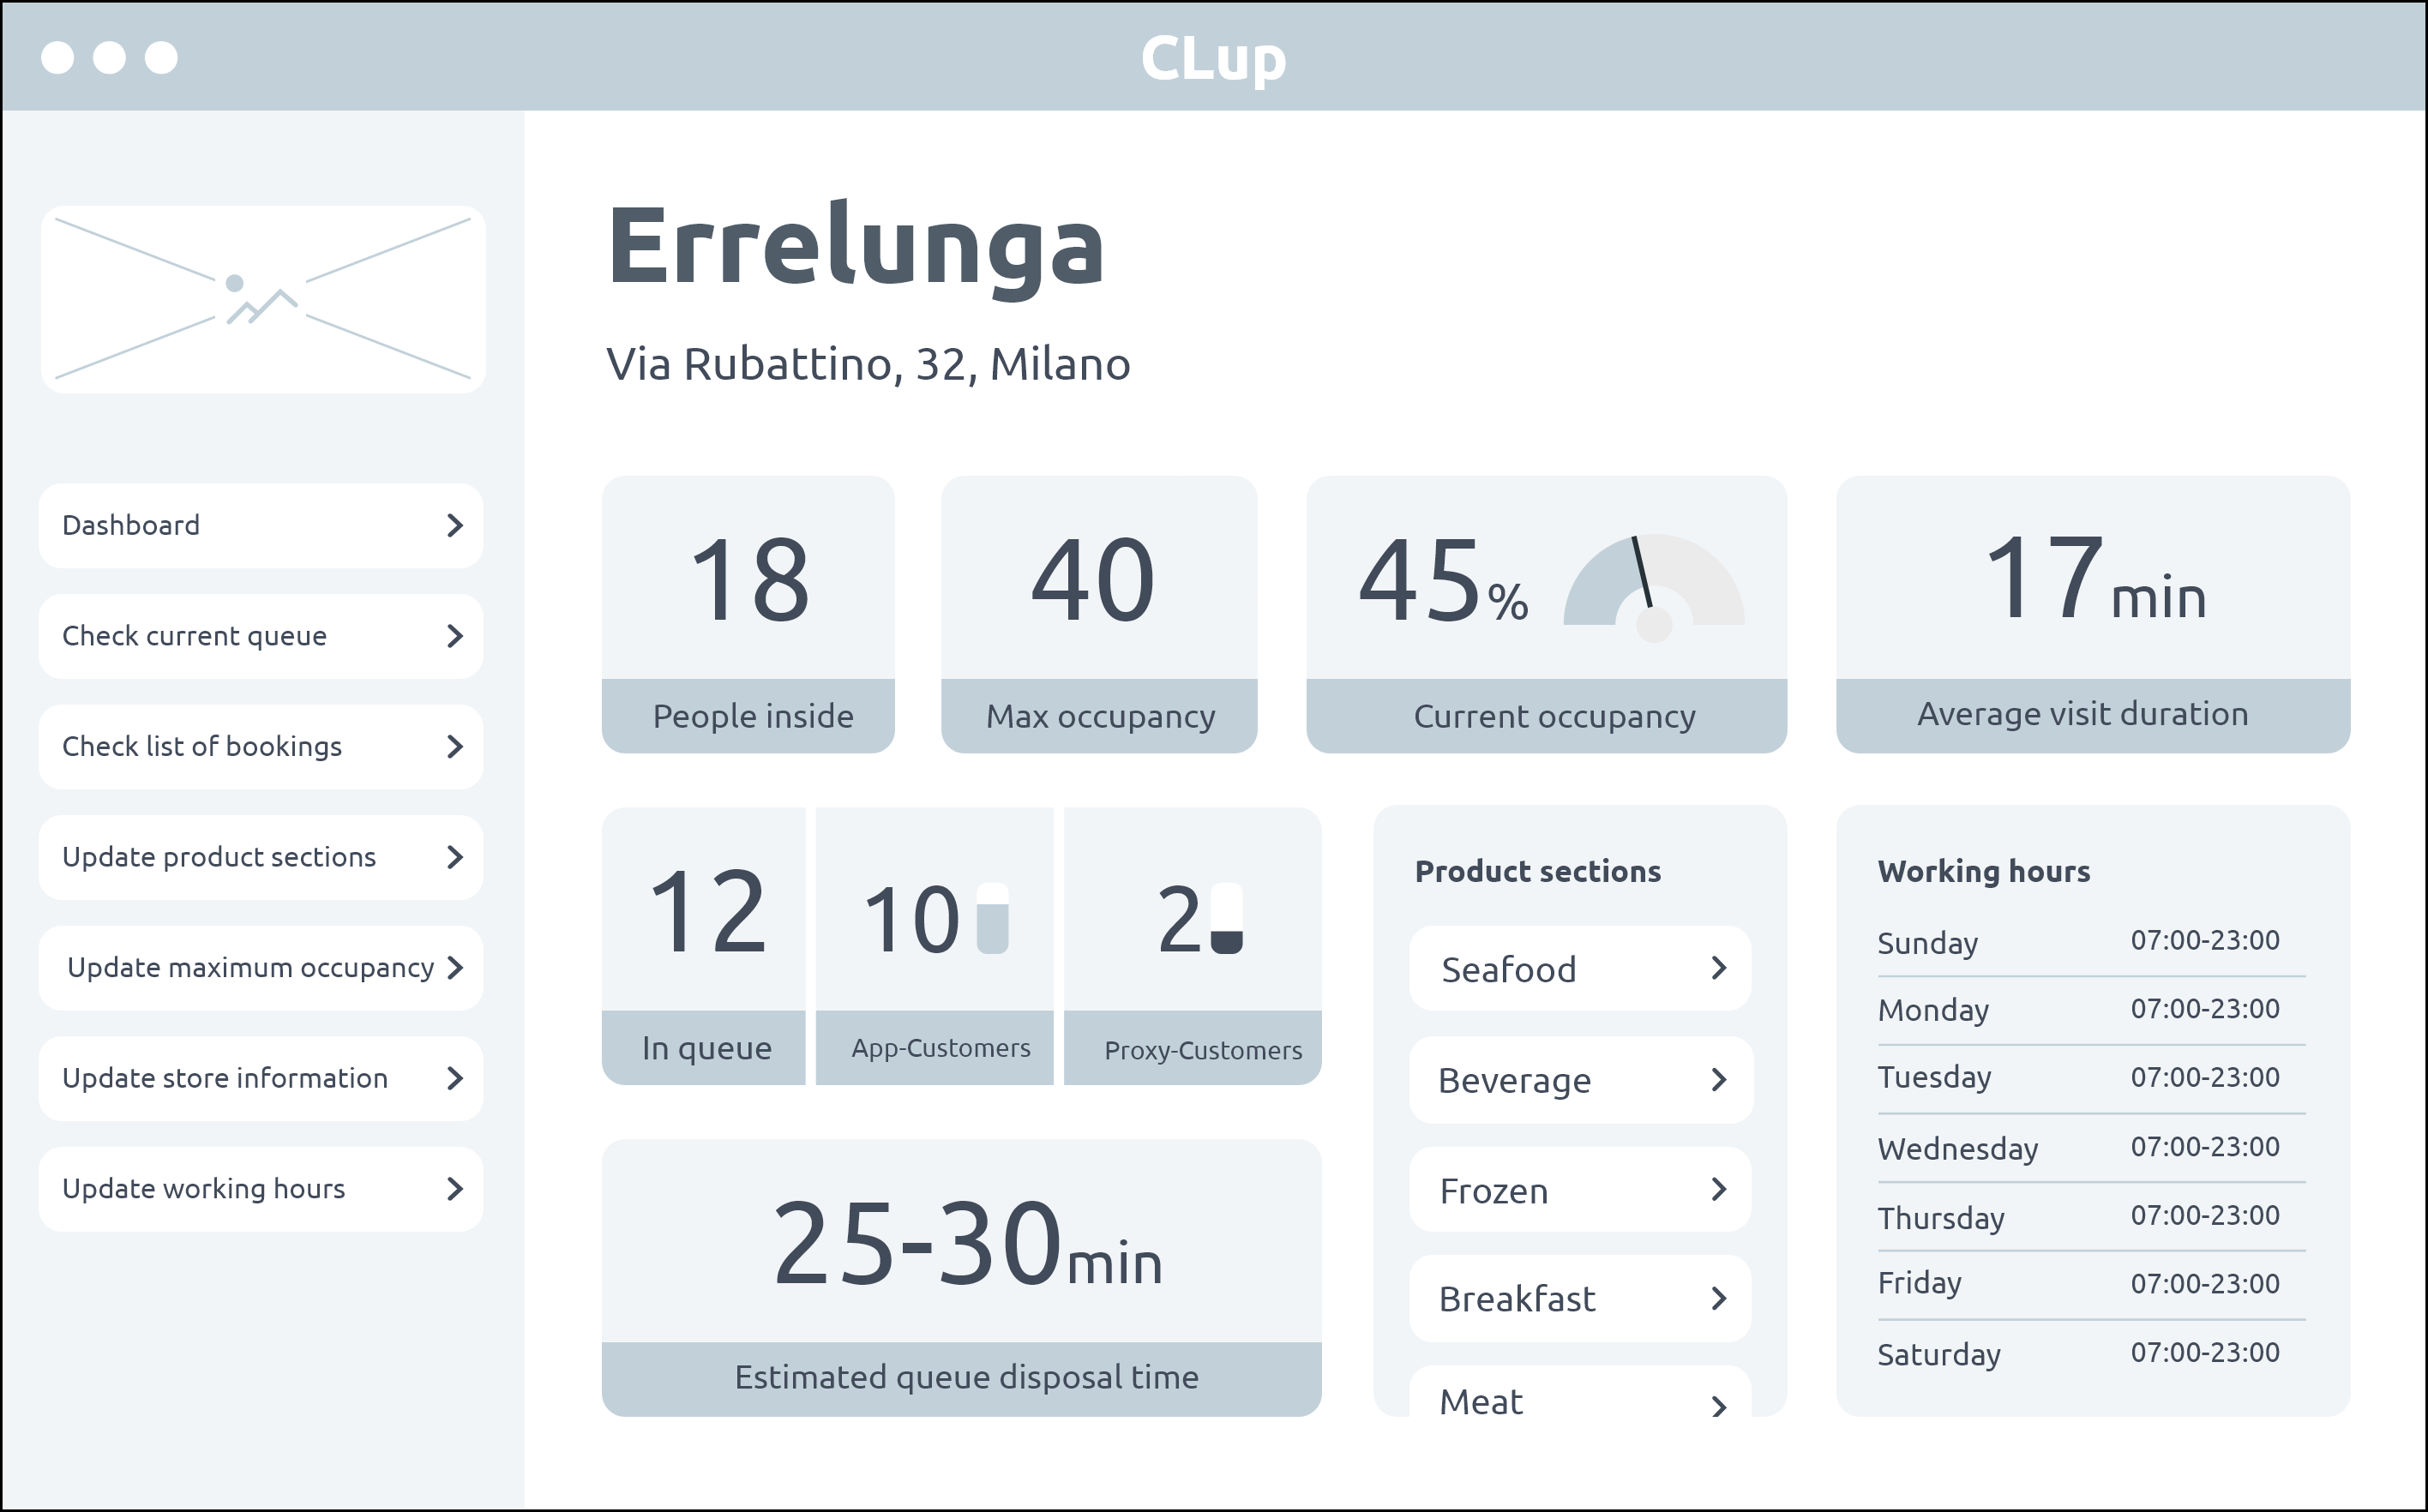
\includegraphics[width=.97\textwidth, height=\textheight, keepaspectratio]{pictures/mockups/manager_view}
        \caption{Mockup 1 -- Manager view}{From his interface, the manager is able to monitor its stores's status. He can also change parameters such as working hours, maximum occupancy and product sections.}
        \label{figure:mockup_1_manager}
    \end{figure}
    
    \begin{figure}[H]
        \centering
        \hspace{0.025\textwidth}
        \begin{minipage}[b]{0.4\textwidth}
            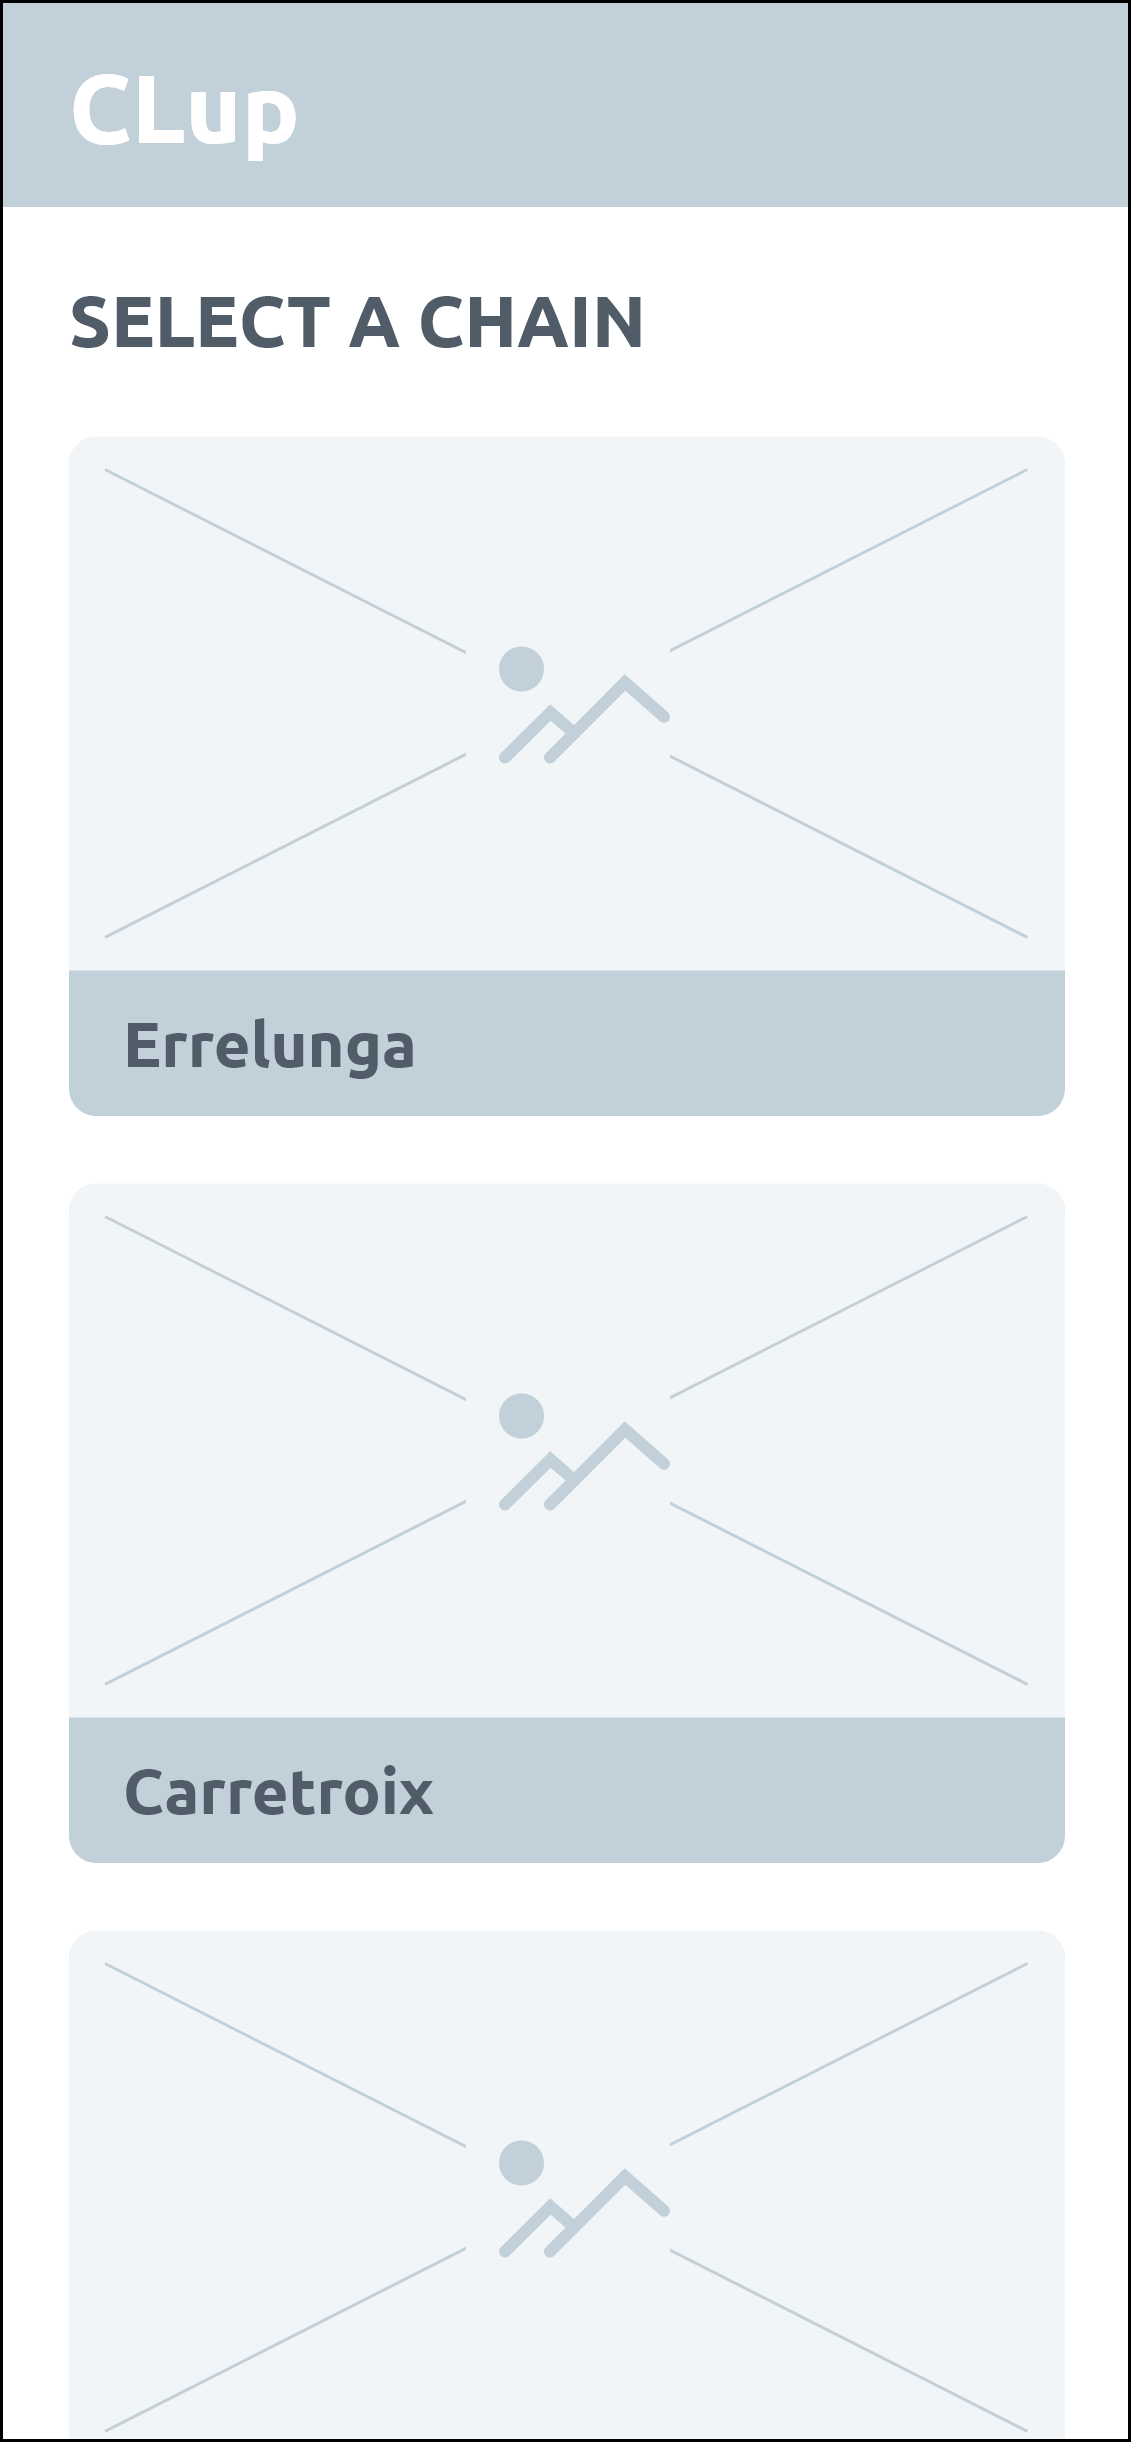
\includegraphics[width=\textwidth]{pictures/mockups/select_chain}
            \captionrasd{Mockup 2 -- Select chain}{A mock-up representing the GUI that the customer sees when he has to select a chain of stores}
        \end{minipage}
        \hspace{0.075\textwidth}
        \begin{minipage}[b]{0.418\textwidth}
            \vspace{-0.5\textheight}
            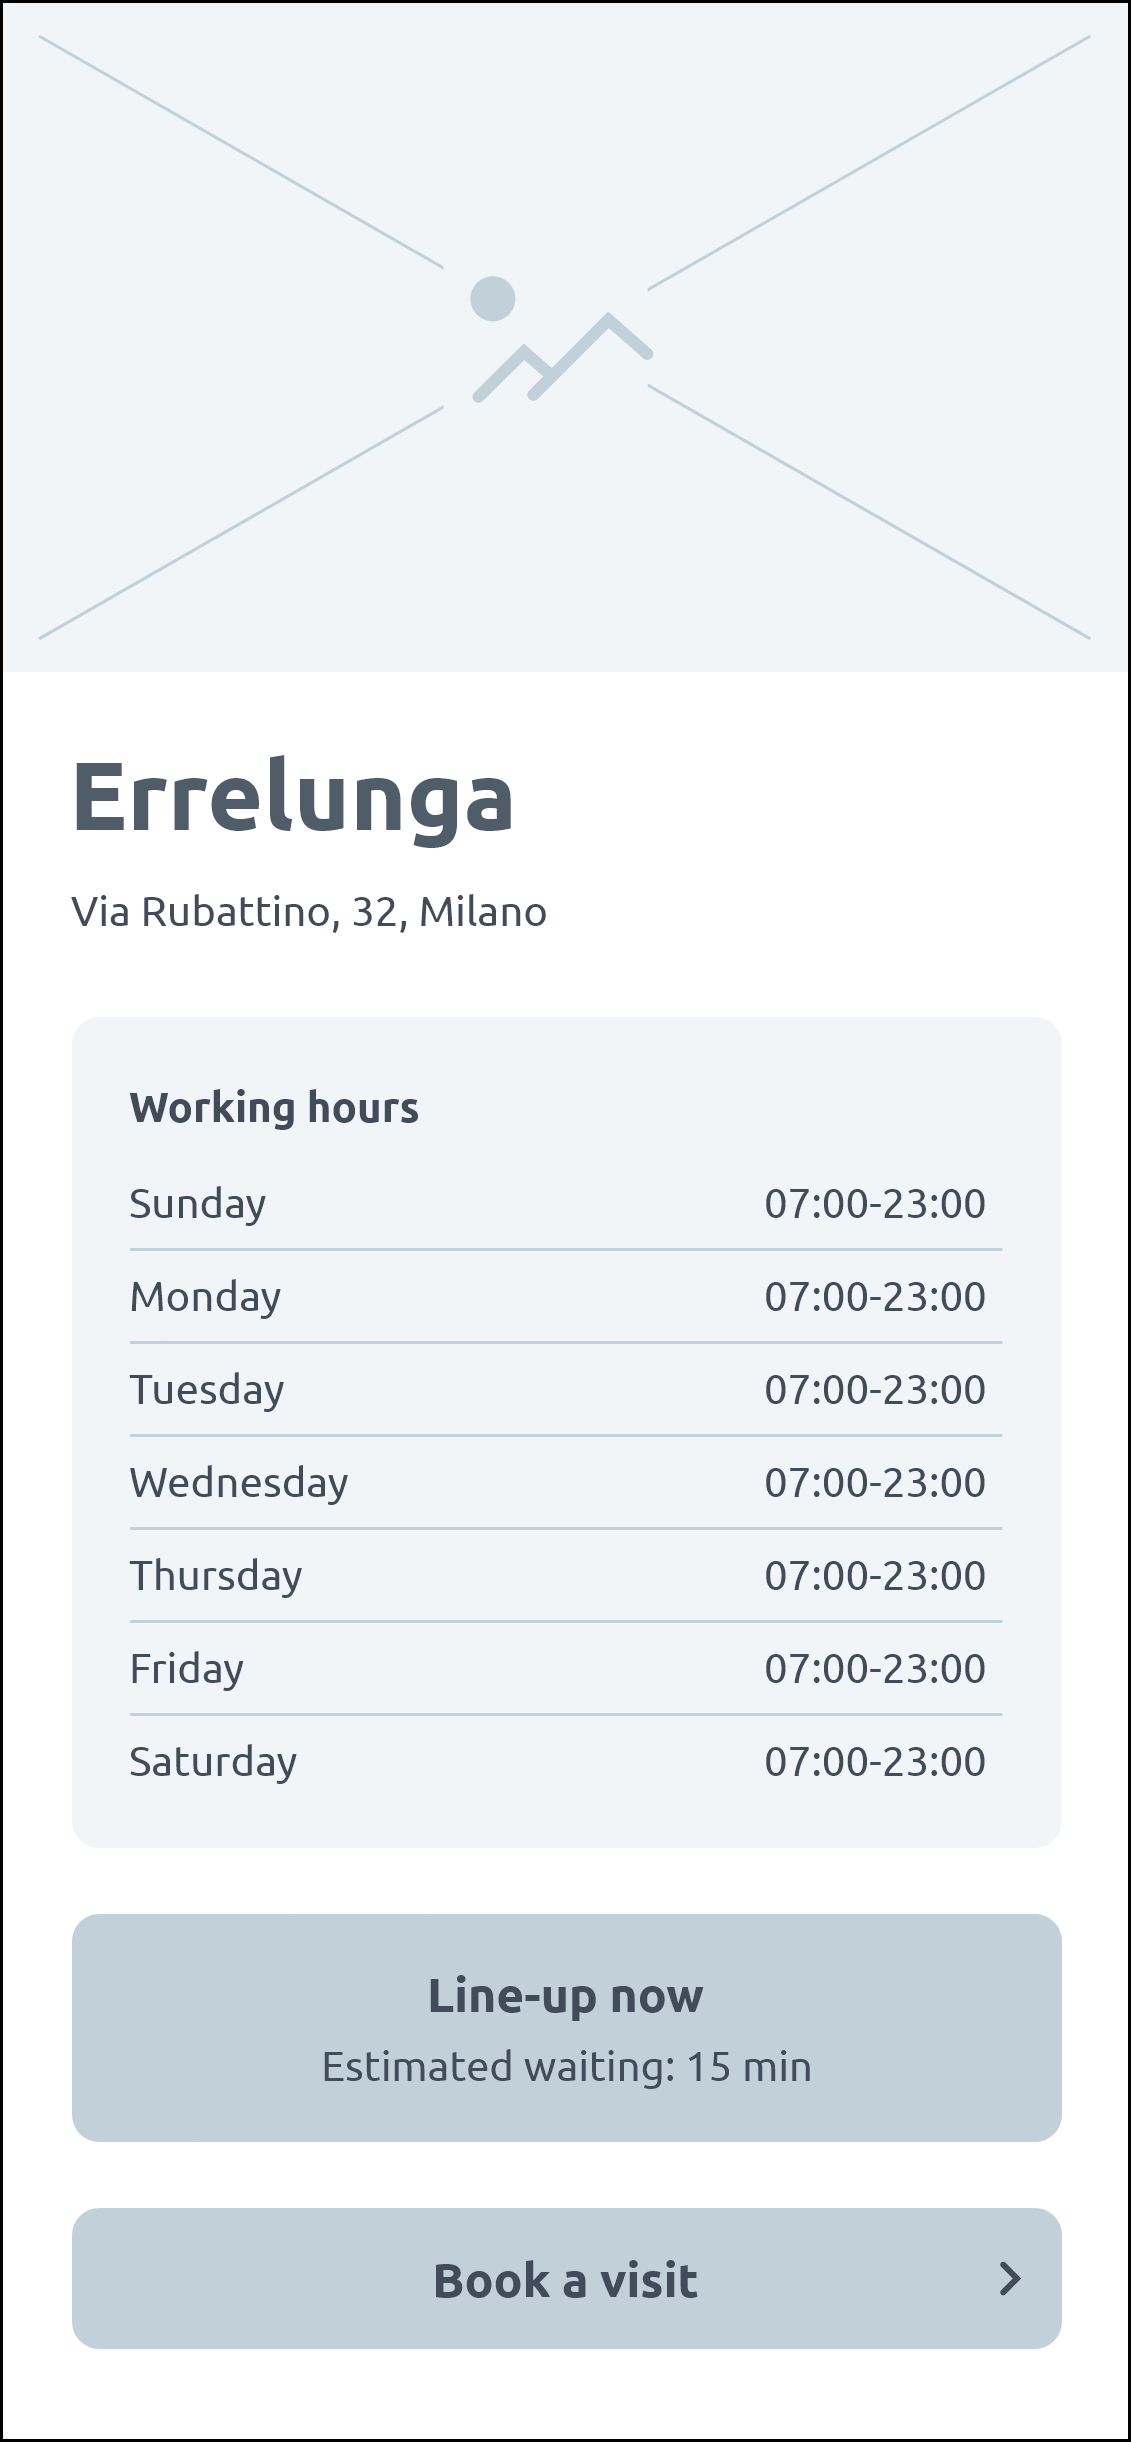
\includegraphics[width=0.958\textwidth]{pictures/mockups/store_view}
            \captionrasd{Mockup 3 -- Store view}{A mock-up representing the GUI that the customer sees when selecting a store}
            \vspace{-0.085cm}
        \end{minipage}
        \hspace{0.025\textwidth}
    \end{figure}

    \subsection{Hardware interfaces}
    \subsubsection{Customer's device} 
    The customer is supposed to use a smartphone to interact with CLup. In order to interact with the system, the smartphone must have an internet connection.
    
    \subsubsection{Manager's device} 
    The manager is supposed to use a personal computer to interact with CLup. In order to interact with the system, it must have an internet connection.
    
    \subsubsection{Proxy} 
    Since the proxy should provide customers with an easy way to line up, it must have at least:
    \begin{itemize}
        \item An internet connection
        \item A way to allows customers to make a line-up request for a single person
        \item A way to physically provide them with the visit token associated with the line-up request
    \end{itemize}
    
    \subsubsection{Turn Announcement System}
    The Turn Announcement System must offer an interface that allows CLup to inform it about the needed information to be provided to the customers. Thus, it must have an internet connection.
    
    \subsubsection{Access Management System}
    The Access Management System must use the API provided by CLup in order to communicate with it and let authorized customers visit the store it belongs to. Thus, it must have an internet connection. The Access Management System must also cope with the case in which the number of people entering the store is less than the number of people specified in the visit request, in order to prevent unauthorized people from entering the store.
    
    \subsection{Software interfaces}
    \subsubsection{Map API}
    In order to properly send notifications, the system must estimate the time needed for the customer to reach the store. Thus, a map service is used to get that estimation based on the customer current position.
    
    \section{Functional requirements}
    \subsection{Table of functional requirements}
    The following requirements refer to a given store of a given chain, both managed by CLup.
    \begin{longtable}[c]{|>{\bfseries{}}c|H{.65\textwidth}|}
        \hline
        \multicolumn{2}{|c|}{\textbf{Functional requirements}} \\
        \hline
        R1   & The system shall allow managers to specify the store parameters \\ \hline
        R2   & The system shall allow managers to monitor entrances \\ \hline
        R3   & The system shall allow managers to monitor exits \\ \hline
        R4   & The system shall authorize accesses to the store \\ \hline
        R4.1 & The system shall authorize customers to enter if and only if the store would not exceed the maximum number of people allowed inside it \\ \hline
        R5   & The system shall provide a way to line up in the virtual queue of the store \\ \hline
        R6   & The system shall provide a way to exit the queue before entering the store \\ \hline
        R7   & The system shall alert the app-customer when it is time to reach the store \\ \hline
        R8   & The system shall provide the possibility to book a time interval for visiting the store \\ \hline
        R9   & The system must not allow customers to book a visit in a time interval if, over its duration, bookings by other users already maximize store occupancy \\ \hline
        R9.1 & The system must not allow customers to book a visit in a time interval if, over its duration, bookings by other users already maximize at least one of the product sections specified in the booking request \\ \hline
        R10  & When booking a visit, the system shall allow customers to specify what kind of products they intend to buy \\ \hline
        R11  & The system shall provide the possibility to cancel a booked visit before entering the store \\ \hline
        R12  & While making a booking request, the system shall suggest alternative time intervals if the demand of the chosen one is too high \\ \hline
        R13  & While making a booking request, the system shall suggest alternative stores of the same chain if the demand for the chosen time interval in the selected store is too high \\ \hline
        R14  & The system shall allow managers to regulate entrances  \\ \hline
        R15  & The system shall allow managers to regulate exits \\ \hline
        R16  & The system shall notify a customer when, during a specific time interval, a specified store is reaching its maximum occupancy \\ \hline
        R17  & The system shall keep track of the average duration of a generic visit to the store \\ \hline
        R18  & The system shall manage the case in which customers do not show up when it is their turn to enter the store \\ \hline
        R19  & The system shall inform customers when they are allowed to enter the store \\ \hline
        \caption{Functional requirements}
        \label{table:functional_requirements}
    \end{longtable}
    
    \newpage
    \subsection{Mapping goals-assumptions-requirements}
    \begin{longtable}[c] { |>{\bfseries{}}c|P{0.22\textwidth}|>{\em}H{0.40\textwidth}| }
        \hline
        \textbf{Goals} & \textbf{Assumptions} & \emph{\textbf{Requirements}} \\
        \hline
        G1 & A2, A2.1, A3, A4, A4.1 & R1, R4, R4.1, R5, R9, R9.1, R10, R12, R13, R14, R15, R18, R19 \\ \hline
        G2 & A1, A4, A5       & R5, R7, R8, R9, R9.1, R12, R13, R17, R18, R19 \\ \hline
        G3 & A1, A4           & R5, R6, R7, R8, R9, R9.1, R11, R12, R13, R16, R17, R18, R19 \\ \hline
        G4 & A3, A4.1         & R1, R2, R3, R14, R15, R17 \\
        \hline
        \caption{Mapping of goals-assumptions-requirements}
        \label{table:map_goals_assumptions_requirements}
    \end{longtable}

    \subsection{Use cases}
    \subsubsection{Use case 1}
    \begin{longtable}[c] { |>{\bfseries{}}C{0.25\textwidth}|H{0.55\textwidth}| }
        \hline
        Name            & Checking the turn \\ \hline
        Actor           & Customer\\ \hline
        Entry condition & The Customer has a visit token \\ \hline
        Event flow      &
        \texttt{1.}The Customer checks if can enter the store \newline
        \texttt{2.}The system provides him with the required information \\\hline 
        Exit condition  & The Customer is aware of whether he can or cannot enter the store \\ \hline
        Exception       & None \\
        \hline
    \caption{Use case 1 -- ``Checking the turn"}
    \label{table:use_case_01}
    \end{longtable}
    
    \subsubsection{Use case 2}
    \begin{longtable}[c] { |>{\bfseries{}}C{0.25\textwidth}|H{0.55\textwidth}| }
        \hline
        Name            & Checking the turn using the application\\ \hline
        Actor           & Customer \\ \hline
        Entry condition & The Customer has a visit token obtained through the application \\ \hline
        Event flow      & 
        \texttt{1.}The Customer opens the application \newline
        \texttt{2.}The Customer checks if he can enter the store for which he made the visit request \newline
        \texttt{3.}The application provides him with the required information \\ \hline
        Exit condition  & The Customer is aware of whether he can or cannot enter the store \\ \hline
        Exception       & None\\
        \hline
    \caption{Use case 2 -- ``Checking the turn using the application"}
    \label{table:use_case_02}
    \end{longtable}
    
    \subsubsection{Use case 3}
    \begin{longtable}[c] { |>{\bfseries{}}C{0.25\textwidth}|H{0.55\textwidth}|}
        \hline
        Name            & Checking the turn in presence \\ \hline
        Actor           & Customer, Turn Announcement System \\ \hline
        Entry condition & The Customer has a visit token \\ \hline
        Event flow      & 
        \texttt{1.}The Customer reaches the store for which he made the visit request \newline
        \texttt{2.}The Customer checks the Turn Announcement System \newline
        \texttt{3.}The Turn Announcement System provides him with the required information obtained by CLup\\ \hline
        Exit condition  & The Customer is aware of whether he can or cannot enter the store \\ \hline
        Exception       & None \\
        \hline
    \caption{Use case 3 -- ``Checking the turn via the Turn Announcement System"}
    \label{table:use_case_03}
    \end{longtable}
    
    \subsubsection{Use case 4}
    \begin{longtable}[c] { |>{\bfseries{}}C{0.25\textwidth}|H{0.55\textwidth}| }
        \hline
        Name            & Visiting the store \\ \hline
        Actor           & Customer, Access Management System \\ \hline
        Entry condition & The Customer is allowed to enter the store. The number of people specified in the visit request is respected  \\ \hline
        Event flow      & 
        \texttt{1.}The Customer moves toward the entrance of the store \newline
        \texttt{2.}The Customer is granted to enter by the external Access Management System using his visit token \newline
        \texttt{3.}The Customer enters the store together with the other people specified in the visit request \newline
        \texttt{4.}The external Access Management System informs CLup that the Customer is inside the store \newline
        \texttt{5.}The Customer does his shopping and is going to exit the store \newline
        \texttt{6.}The Customer is granted to exit by the external Access Management System using his visit token \newline
        \texttt{7.}The Customer exits the store together with the other people specified in the visit request \newline
        \texttt{8.}The external Access Management System informs CLup that the Customer has exited the store
        \\ \hline
        Exit condition  & CLup is aware of the actual number of people inside the store \\ \hline
        Exception       & Different exceptions can arise: \newline
        -- The Customer is not yet allowed to enter the store \newline
        -- The Customer has lost or does not have access to his visit token. If the Customer is not already in the store, he loses the possibility to enter. If the Customer is already in the store, he can exit it only with the help of a store manager \newline
        -- The Customer does not show up \\
        \hline
    \caption{Use case 4 -- ``Visiting the store"}
    \label{table:use_case_04}
    \end{longtable}
    
    \subsubsection{Use case 5}
    \begin{longtable}[c] { |>{\bfseries{}}C{0.25\textwidth}|H{0.55\textwidth}| }
        \hline
        Name            & Place a visit request \\ \hline
        Actor           & Customer \\ \hline
        Entry condition & The Customer wants to visit a store \\ \hline
        Event flow      & 
        \texttt{1.}The Customer chooses to line up or to book a visit \newline
        \texttt{2.}The Customer uses the dedicated function provided by CLup \newline
        \texttt{3.}The Customer receives a visit token\\ \hline
        Exit condition  & The Customer has what he needs to access the store \\ \hline
        Exception       & Exceptions can arise while lining up or booking a visit \\
        \hline
    \caption{Use case 5 -- ``Place a visit request"}
    \label{table:use_case_05}
    \end{longtable}
    
    \subsubsection{Use case 6}
    \begin{longtable}[c] { |>{\bfseries{}}C{0.25\textwidth}|H{0.55\textwidth}| }
        \hline
        Name            & Place a line-up request (lining up) \\ \hline
        Actor           & Customer \\ \hline
        Entry condition & The Customer wants to line up for a store and the store is open \\ \hline
        Event flow      & 
        \texttt{1.}The Customer interacts with one of the interfaces provided to him by CLup. He can use both the application or the proxy. If the Customer uses the application, he also selects the desired chain and store \newline
        \texttt{2.}The Customer uses the function to line up offered by CLup. In case of app-customers, they also indicate the number of people who want to visit the store \newline
        \texttt{3.}An access request is generated with an associated visit token, which is provided to the Customer \newline 
        \texttt{4.}The Customer receives the visit token \\ \hline
        Exit condition  & The Customer has what he needs to access the store \\ \hline
        Exception       & The visit request cannot be generated. This can happen due to different causes: \newline
        -- a communication error occurs \newline
        -- the store is closed \newline
        An error is shown to the Customer and the lining up operation is not completed \\
        \hline
    \caption{Use case 6 -- ``Place a line-up request (lining up)"}
    \label{table:use_case_06}
    \end{longtable}
    
    \newpage
    \subsubsection{Use case 7}
    \begin{longtable}[c] { |>{\bfseries{}}C{0.25\textwidth}|H{0.55\textwidth}| }
        \hline
        Name            & Booking a visit (place a booking request) \\ \hline
        Actor           & Customer \\ \hline
        Entry condition & The Customer wants to book a visit to a store \\ \hline
        Event flow      & 
        \texttt{1.}The Customer opens the application and selects the desired chain and store \newline
        \texttt{2.}The Customer selects the function for booking a visit \newline
        \texttt{3.}The Customer receives information about the store from CLup, such as the product sections and the personal estimated visit duration, if available \newline
        \texttt{4.}The Customer specifies when he wants to enter the store \newline
        \texttt{5.}The Customer specifies the estimated duration of the visit. If he is a long-term customer, an approximate duration is suggested by CLup \newline
        \texttt{6.}The Customer can specify which kind of products he intends to buy \newline
        \texttt{7.}The Customer specifies the number of additional people who wants to visit the store with him  \newline
        \texttt{8.}The Customer confirms that he wants to book a visit \newline
        \texttt{9.}A booking is generated and a visit token is associated to it \newline
        \texttt{10.}The Customer receives the visit token \\ \hline
        Exit condition  & The Customer has what he needs to access the store \\ \hline
        Exception       & Different exceptions can arise: \newline
        -- The selected store is closed during the time interval specified by the Customer \newline
        -- The store has already reached its maximum occupancy during the chosen time interval. Then the application suggests alternative time intervals or alternative available stores of the same chain. However, if the Customer does not specify a different time interval or a different store he cannot place the booking \newline
        -- The store is likely to reach its maximum occupancy during the chosen time interval. Then the application suggests an alternative time interval or other stores of the same chain in order to balance the number of people inside the store selected by the Customer. However, the Customer can book the visit anyway \newline
        -- A communication problem occurs after step 6 \newline
        An error is shown to the Customer and the booking operation is not completed \\
        \hline
    \caption{Use case 7 -- ``Booking a visit (place a booking request)"}
    \label{table:use_case_07}
    \end{longtable}
    
    \subsubsection{Use case 8}
    \begin{longtable}[c] { |>{\bfseries{}}C{0.25\textwidth}|H{0.55\textwidth}| }
        \hline
        Name            & Reaching the store \\ \hline
        Actor           & Customer \\ \hline
        Entry condition & The Customer who used the application to request the visit should now head to the store if he wants to arrive in time  \\ \hline
        Event flow      & 
        \texttt{1.}CLup retrieves the Customer’s position \newline
        \texttt{2.}Considering the distance between his position and the store, a notification is sent to the Customer when he should head to the store in order to arrive in time. This is done with respect to the estimated time in which the Customer should be able to enter the store \newline
        \texttt{3.}The Customer reads the notification \\ \hline
        Exit condition  & The Customer is aware that he should head to the store \\ \hline
        Exception       & The Customer location cannot be sent to CLup. Possible causes: \newline
        -- the position is not available \newline
        -- a communication error occurs \newline
        For this reason, no notification is sent \\
        \hline
    \caption{Use case 8 -- ``Reaching the store"}
    \label{table:use_case_08}
    \end{longtable}
    
    \subsubsection{Use case 9}
    \begin{longtable}[c] { |>{\bfseries{}}C{0.25\textwidth}|H{0.55\textwidth}| }
        % \hline \multicolumn{2}{|c|}{\textbf{Checking the turn}} \\
        \hline
        Name            & The store is filling up \\ \hline
        Actor           & Customer \\ \hline
        Entry condition & The Customer expresses the will to be notified about the availability of a store in specific time intervals \\ \hline
        Event flow      & 
        \texttt{1.}The information about the store and the time interval the Customer wants to be notified about is either inferred by CLup or specified by the Customer himself \newline
        \texttt{2.}That time interval is likely to be saturated (i.e. no other bookings in that time interval are going to be allowed or the current estimated disposal time of the queue is going to reach the end of the time interval) \newline
        \texttt{3.}CLup notifies the Customer about it \\ \hline
        Exit condition  & The Customer is aware that the store is reaching its maximum occupancy during the time intervals he is interested in \\ \hline
        Exception       & None \\
        \hline
    \caption{Use case 9 -- ``The store is filling up"}
    \label{table:use_case_09}
    \end{longtable}
    
    \subsubsection{Use case 10}
    \begin{longtable}[c] { |>{\bfseries{}}C{0.25\textwidth}|H{0.55\textwidth}| }
        \hline
        Name            & Administering the store \\ \hline
        Actor           & Manager \\ \hline
        Entry condition & The Manager wants to edit some parameters of one of the stores he manages \\ \hline
        Event flow      & 
        \texttt{1.}The manager uses the tool to check the current status of the store \newline
        \texttt{2.}If needed, the manager adjusts store parameters \newline \\ \hline
        Exit condition  & The Manager is aware of the status of the store and CLup is up to date with Manager choices \\ \hline
        Exception       & The parameters specified by the Manager are not valid \\
        \hline
    \caption{Use case 10 -- ``Administering the store"}
    \label{table:use_case_10}
    \end{longtable}
    
    \subsubsection{Use case 11}
    \begin{longtable}[c] { |>{\bfseries{}}C{0.25\textwidth}|H{0.55\textwidth}| }
        \hline
        Name            & Let a customer exit the store \\ \hline
        Actor           & Customer, Manager, Access Management System \\ \hline
        Entry condition & The Customer has asked the Manager to exit the store because he has lost his visit token \\ \hline
        Event flow      & 
        \texttt{1.}The Manager uses the administrative tool to allow the Customer to exit the store \newline
        \texttt{2.}The Customer exits the store by means of the Access Management System \newline
        \texttt{3.}CLup updates the store occupancy \\ \hline
        Exit condition  & CLup is aware of the actual number of people in the store. The Customer has left the store \\ \hline
        Exception       & None \\
        \hline
    \caption{Use case 11 -- ``Let a customer exit the store"}
    \label{table:use_case_11}
    \end{longtable}
    
    \subsubsection{Use case 12}
    \begin{longtable}[c] { |>{\bfseries{}}C{0.25\textwidth}|H{0.55\textwidth}| }
        \hline
        Name            & Cancel visit \\ \hline
        Actor           & Customer \\ \hline
        Entry condition & The Customer has a visit token and is not already in the store \\ \hline
        Event flow      & 
        \texttt{1.}The Customer asks CLup to delete a visit request he made before \newline
        \texttt{2.}CLup processes and deletes the request \\ \hline
        Exit condition  & The Customer’s visit token is not valid anymore \\ \hline
        Exception       & None \\
        \hline
    \caption{Use case 12 -- ``Cancel visit"}
    \label{table:use_case_12}
    \end{longtable}
    
    \subsection{Use case diagram}
    \begin{figure}[H]
        \centering
        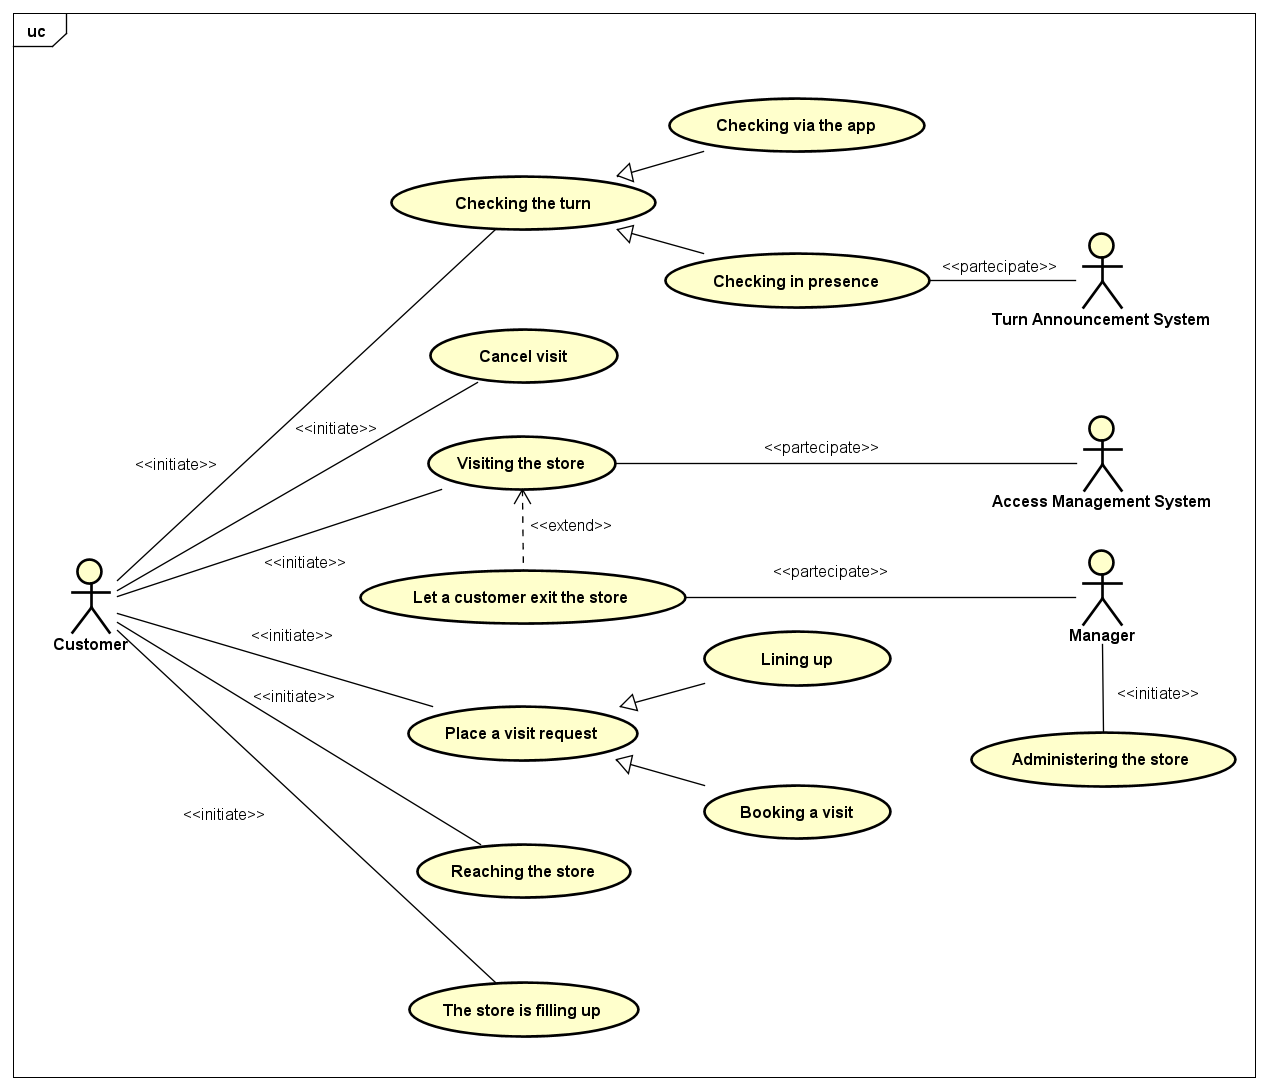
\includegraphics[width=\textwidth, height=\textheight, keepaspectratio]{pictures/use_case_diagram}
        \caption{Use case diagram}
        \label{figure:use_case_diagram}
    \end{figure}
    
    \newpage
    \subsection{Sequence Diagrams}
    The following diagrams are some of the most significant Sequence Diagrams, and each of them refers to the homonym Use Case. 
    
    \begin{figure}[H]
        \centering
        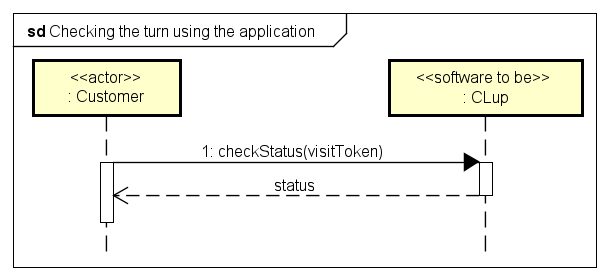
\includegraphics[width=0.85\textwidth, keepaspectratio]{pictures/sequence_diagrams/check_turn_via_app}
        \captionrasd{Sequence diagram 1 -- ``Checking the turn using the application"}{This sequence diagram shows the interaction between an app-customer checking the turn and CLup}
        
        \label{figure:sequence_diagram_1_check_turn_via_app}
    \end{figure}
    
    \begin{figure}[H]
        \centering
        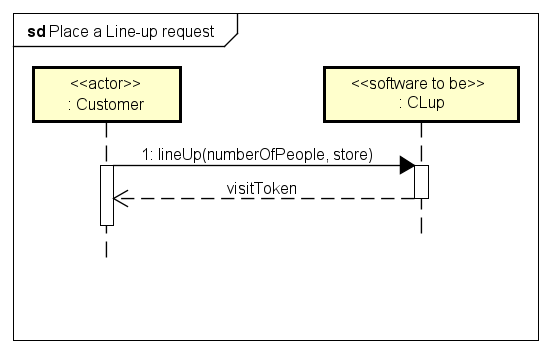
\includegraphics[width=0.85\textwidth, keepaspectratio]{pictures/sequence_diagrams/place_line-up_request}
        \captionrasd{Sequence diagram 2 -- ``Place a line-up request"}{Sequence diagram shows the interaction between a customer who lines up and CLup}
        \label{figure:sequence_diagram_2_place_lineup_request}
    \end{figure}
    
    \begin{figure}[H]
        \centering
        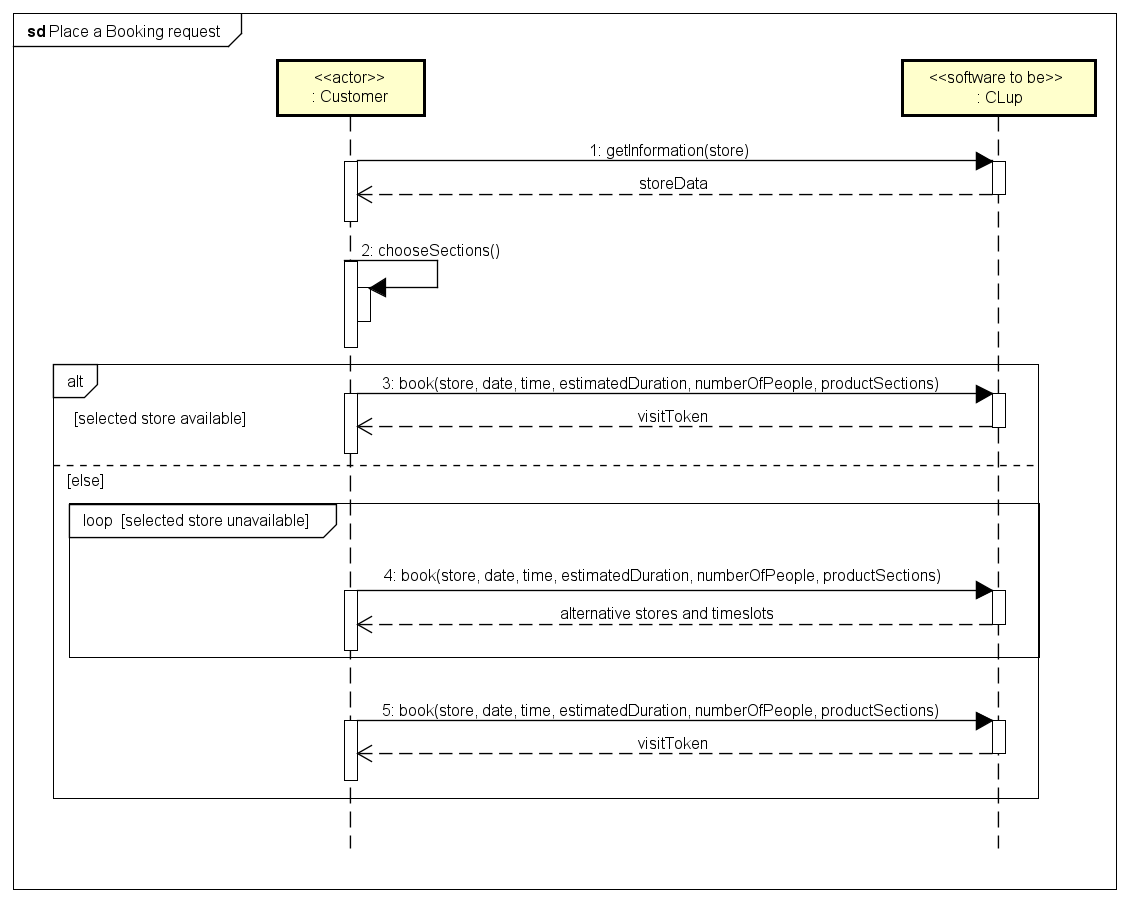
\includegraphics[width=0.95\textwidth, keepaspectratio]{pictures/sequence_diagrams/place_booking_request}
        \captionrasd{Sequence diagram 3 -- ``Place a booking request"}{This sequence diagram shows the interaction between an app-customer placing a booking request and CLup}
        \label{figure:sequence_diagram_3_place_booking_request}
    \end{figure}
    
    \begin{figure}[H]
        \centering
        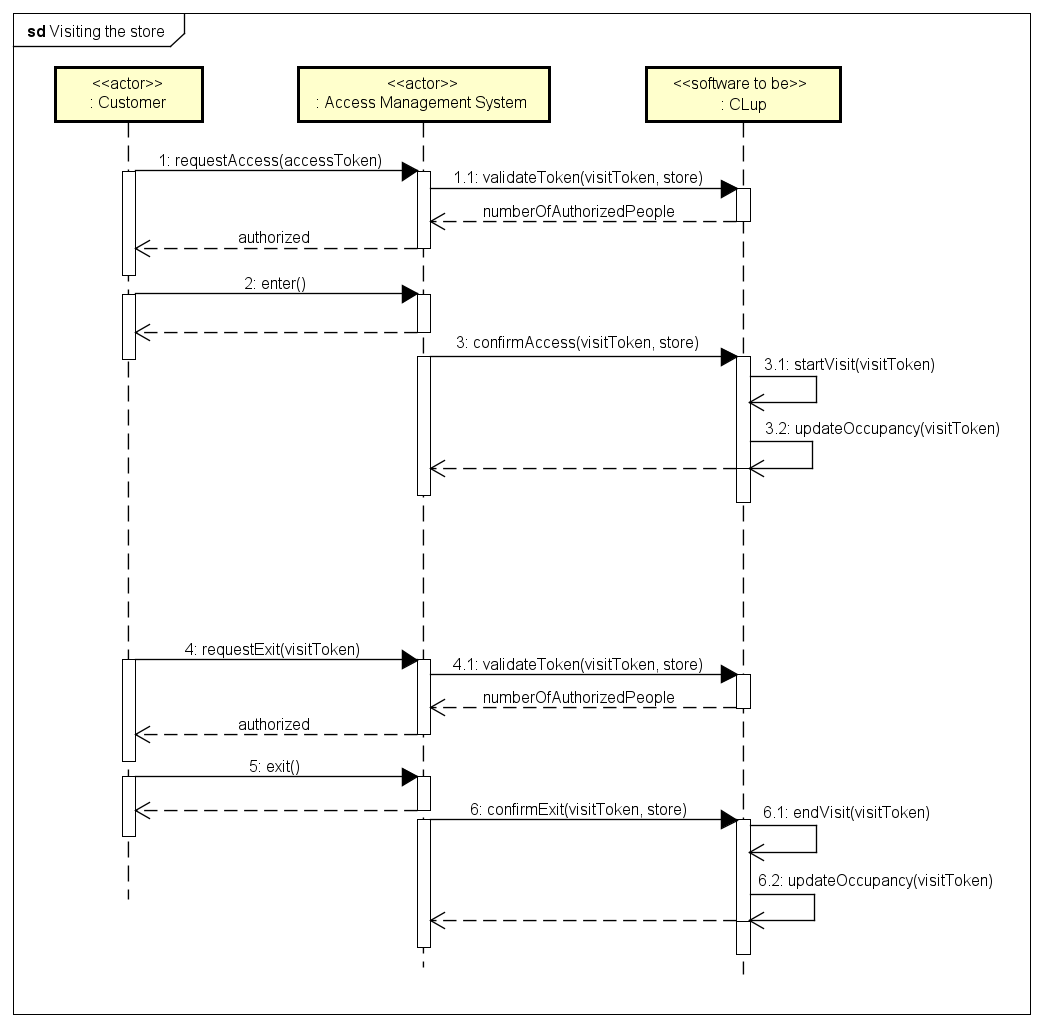
\includegraphics[width=0.95\textwidth, keepaspectratio]{pictures/sequence_diagrams/visiting_the_store}
        \captionrasd{Sequence diagram 4 -- ``Visiting the store"}{This sequence diagram illustrates the dynamic behaviour of the system when a customer visits the store}
        \label{figure:sequence_diagram_4_visiting_store_app}
    \end{figure}
    
    \newpage
    \subsection{Activity diagrams}
    The following activity diagrams represent the interaction between both app-customers and proxy-customer with the system.
    
    \begin{figure}[H]
        \centering
        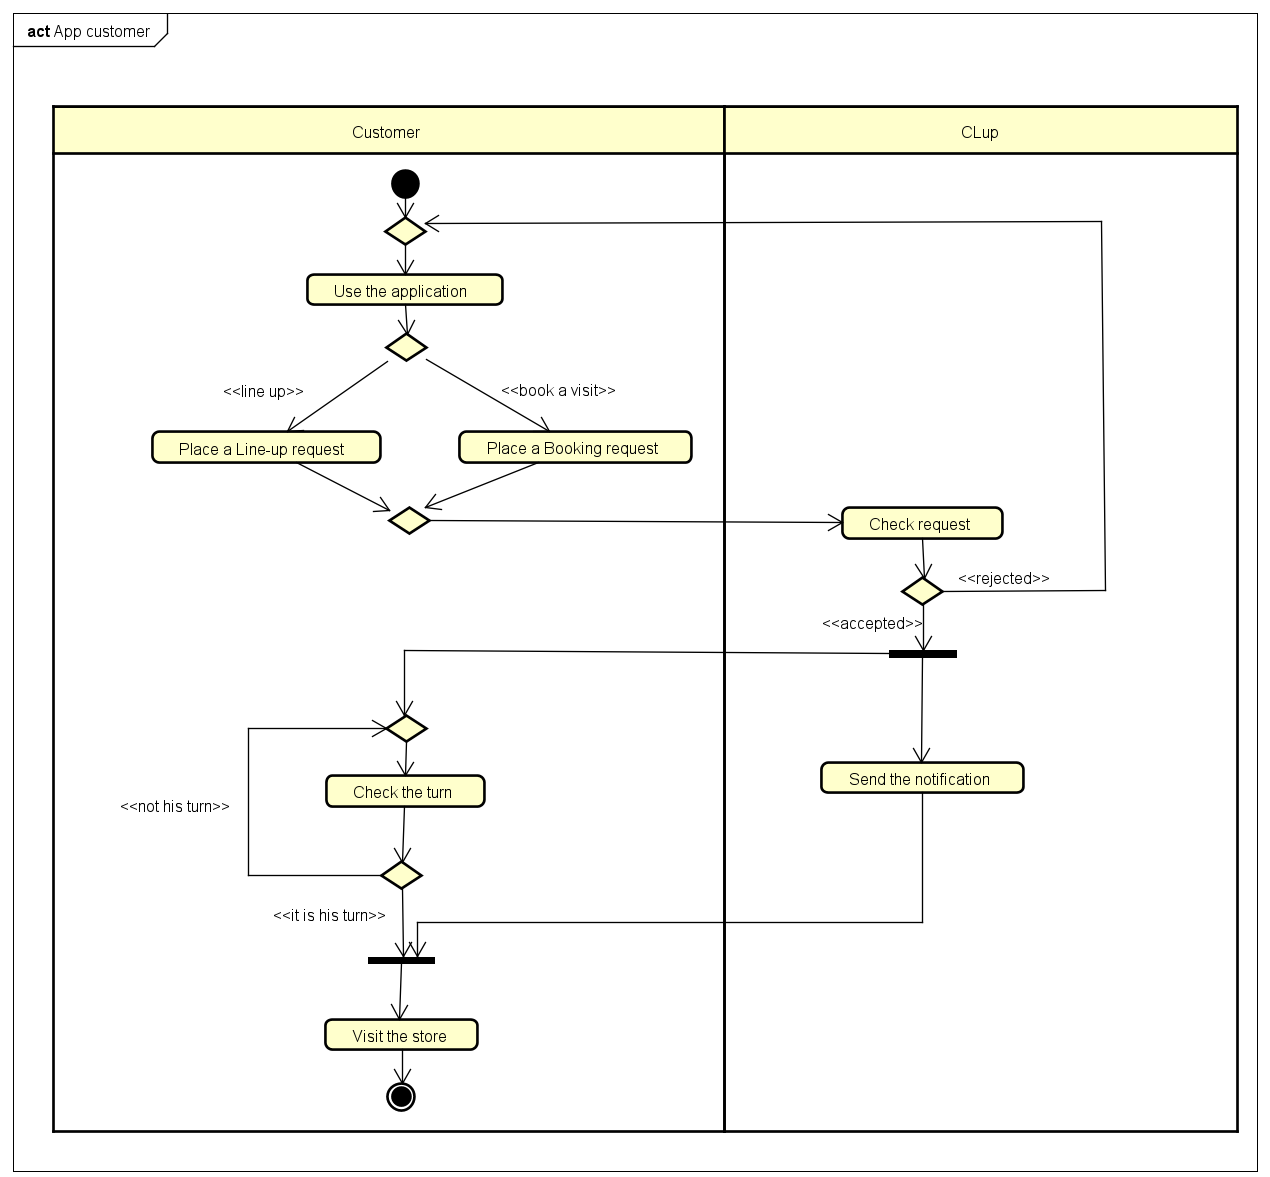
\includegraphics[width=0.9\textwidth, keepaspectratio]{pictures/activity_diagrams/app_customer}
        \captionrasd{Activity diagram 1 -- ``App customer"}{This activity diagram shows the flow of events related to a customer who uses the application and wants to visit the store}
        \label{figure:activity_diagram_1_app_customer}
    \end{figure}
    
    \begin{figure}[H]
        \centering
        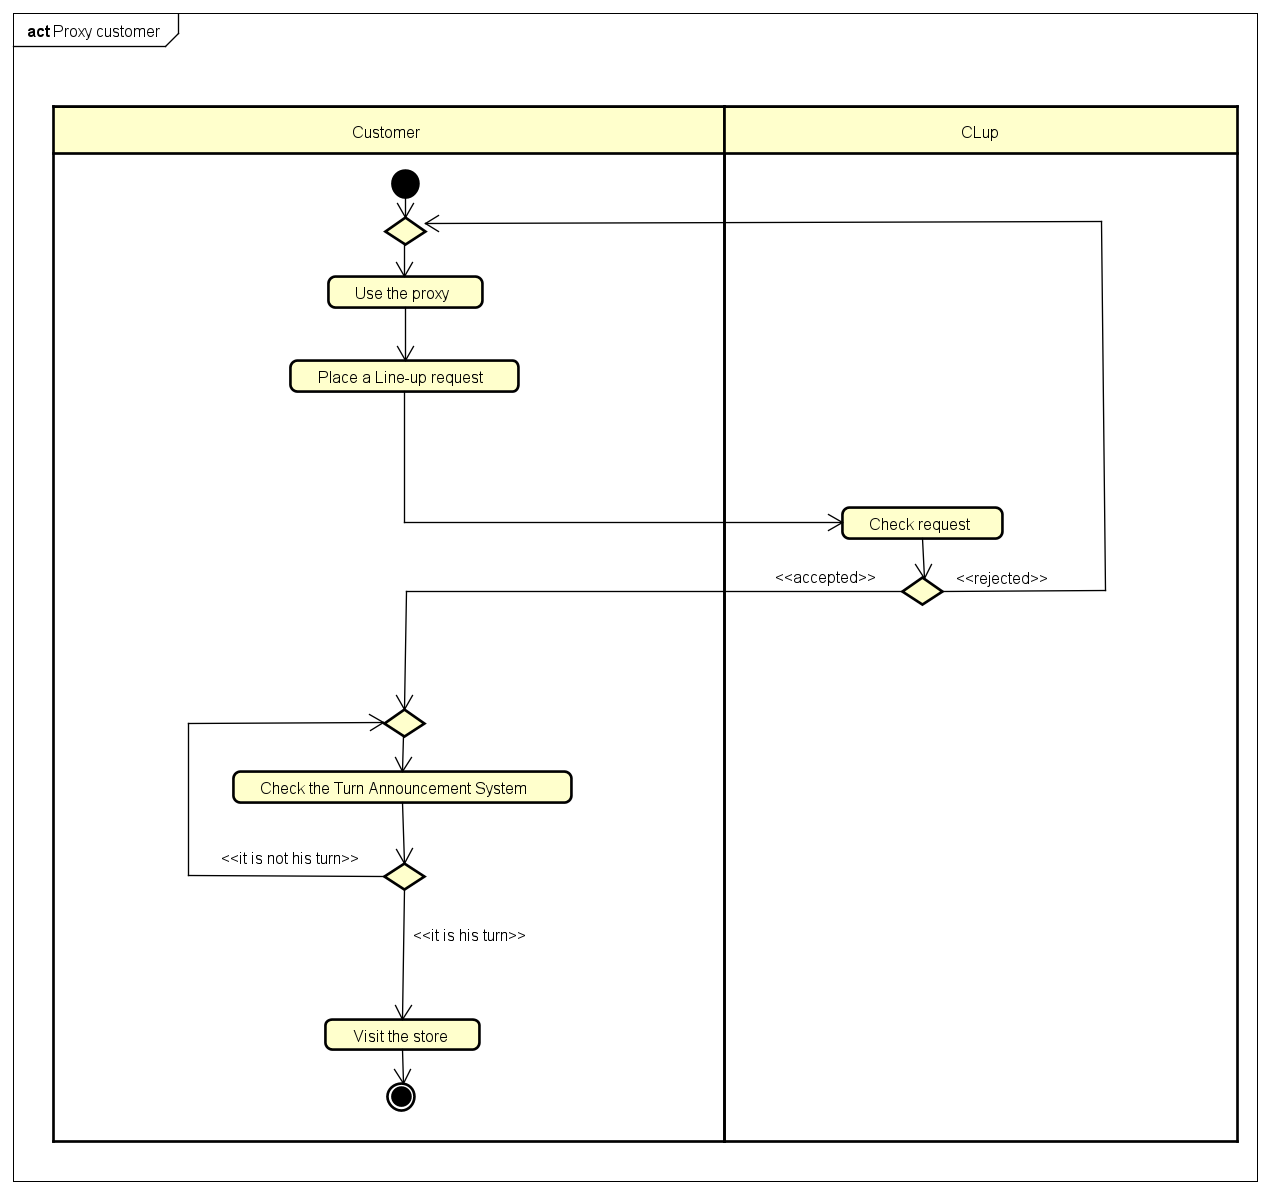
\includegraphics[width=0.9\textwidth, keepaspectratio]{pictures/activity_diagrams/proxy_customer}
        \captionrasd{Activity diagram 2 -- ``Proxy customer''}{This activity diagram shows the flow of events related to a customer who uses the proxy and wants to visit the store}
        \label{figure:activity_diagram_1_proxy_customer}
    \end{figure}
    
    \subsection{Traceability}
    \begin{longtable}[c] { |>{\bfseries{}}c|H{0.32\textwidth}|H{.45\textwidth}| }
        \hline
        Goal & \textbf{Requirements} & \textbf{Use cases} \\
        \hline
        G1 & R1, R4, R4.1, R5, R9, R9.1, R10, R12, R13, R14, R15, R18 & UC1, UC2, UC3, UC4, UC5, UC6, UC7, UC11 \\ \hline
        G2 & R5, R7, R8, R9, R9.1, R12, R13, R17, R18, R19 & UC1, UC2, UC3, UC5, UC6, UC7, UC8 \\ \hline
        G3 & R5, R6, R7, R8, R9, R9.1, R11, R12, R13, R16, R17, R18, R19 & UC1, UC2, UC5, UC6, UC7, UC8, UC9, UC12 \\ \hline
        G4 & R1, R2, R3, R14, R15, R17 & UC4, UC10, UC11 \\
        \hline
        \caption{Traceability matrix}
        \label{table:traceability_matrix}
    \end{longtable}
    %%%%%%%%%%%%%%%%%%%%%%%%%%%%
    
    \section{Performance requirements}
    The system, in normal operating conditions, should be able to handle all line-up and booking requests of each customer. It should be able to manage, without a loss in performance, a large number of simultaneous visit requests which, in a non optimal case, are likely to be in the order of the sum of all maximum occupancies of each store managed by CLup. \par
    The system responses and notifications must be sent within 3 seconds from the triggering event.
    
    \section{Design constraints}
    \subsection{Standard compliance}
    The whole software should be compliant with the General Data Protection Regulation (GDPR).
    
    \section{Software system attributes}
    \subsection{Reliability}
    The context in which CLup operates is characterized by a strong focus on safety and distancing between people. Thus, the system must guarantee a high degree of reliability in order to prevent dangerous situations in which safety constraints are violated both inside and outside the store. 
    
    \subsection{Availability}
    In order to help the store manager to regulate the influx of people to the store and prevent gatherings, CLup should be available the 99\% of the time.
    
    \subsection{Security}
    The system should focus on protecting against attacks which affect its availability and reliability. It is also fundamental to protect both customers and managers from man-in-the-middle attacks. They should exchange messages and information only with CLup, while keeping private information safe (e.g. customer’s current position and future movements).
    
    CLup shall also identify all of the store managers before allowing them to use the store administrative tool.
    
    \subsection{Maintainability}
    Over time, the system could need corrections, improvements and additions. For this reason, the system must be well-documented and adaptable to changes.
    
    \subsection{Portability}
    The CLup customer application should be compatible with most of the smartphones currently on the market. This way, everyone can benefit from the system, save time and avoid crowding by queuing remotely and by booking visits. The same should apply for the administrative tool provided to managers, which should be compatible with most of the currently available computers on the market.\par
    Moreover, CLup should be platform independent in order to increase degrees of freedom when choosing the hardware to use and when defining its possible future upgrades.
    
    \subsection{Accessibility}
    The application should be easy to use, in order to allow all the different possible customers to visit the store.
    
    \section{Other requirements}
    \begin{itemize}
        \item CLup shall give priority to booking requests over line-up requests; \item Customers can remotely line up in a store’s queue only if they are not in the queue of any store at that moment;  
        \item Customers can book a visit for a specific time interval only if they have not booked any other visit which overlaps with that time interval;
        \item Customers can book a visit to a store and for a specific time interval only if it starts after the current queue disposal time of that store.
    \end{itemize}
   

\chapter{Alloy}
    \section{Alloy description}
    The Alloy model presented below aims to show how it is possible to build a coherent and consistent solution to the problem explained in this document, taking into account all the already specified constraints. To do so, the Alloy model neglects some aspects of the UML that are not strictly useful to do this kind of analysis, while focusing on the principal behaviours of the system. \par
    As it can be seen by executing the “show” predicate, which includes some constraints of convenience on the number of instances of some signatures, all the specified facts allow to build a feasible instance of the problem that is coherent with all the requirements and constraints. \par
    For the sake of simplicity, time intervals and time in general are represented using integers, and the behaviour of product sections with respect to their maximum occupancy is not deeply investigated. Furthermore, the signatures “Date” and “Token” are not deeply characterized for the same simplicity reasons. \par
    In particular, the model shows that:
    \begin{itemize}
        \item a visit can take place only after its request has been placed;
        \item a customer can line-up only for a store at a time;
        \item a customer cannot visit more than one store at the same time;
        \item a customer cannot book two overlapping time intervals among all the stores;
        \item it is not possible to book a visit if that booking would make the store exceed its maximum occupancy;
        \item it is not possible to book a visit which does not fits in the store working hours;
        \item it is not possible to book a visit that starts before the current queue disposal time;
        \item it is not possible to line up when the store is closed;
        \item the current store occupancy is the number of people in the store at that moment;
        \item tokens, manager ids and product sections are unique.
    \end{itemize}

    \section{Alloy model}
    \begin{lstlisting}[language=alloy]
sig Date {}
sig TimeInterval {
    start : Int,
    end   : Int
} {
    start >= 0 and
    start < end
}
sig Token {} {
    Token = Visit_Request.visit_token
}

sig ID {} {
    ID = Manager.id
}

sig Manager {
    id     : ID,
    stores : some Store
}

sig Chain {
    stores : some Store
}

sig Store {
    parent_chain      : Chain,
    current_occupancy : Int,
    maximum_occupancy : Int,
    working_hours     : some TimeInterval,
    sections          : some Product_Section,
    visit_request 	  : set Visit_Request,
    queue             : Queue,
    managers          : some Manager
} {
    current_occupancy >= 0 and
    current_occupancy <= maximum_occupancy
}

sig Queue {
    store                   : Store,
    length                  : Int,
    estimated_disposal_time : Int,
    requests                : set LineUp_Request
} {
    estimated_disposal_time >= 0 and
    length = #requests
}

sig Product_Section {
    store             : Store,
    current_occupancy : Int,
    maximum_occupancy : Int
} {
    current_occupancy >= 0 and
    maximum_occupancy >  0 and
    current_occupancy <= maximum_occupancy
}

abstract sig Visit_Request {
    store            : Store,
    number_of_people : Int,
    date_of_creation : Date,
    time_of_creation : Int,
    visit_token      : Token,
    customer         : Customer,
    visit			 : lone Visit
} {
    number_of_people > 0 and
    time_of_creation >= 0
}

sig LineUp_Request extends Visit_Request {
}

sig Booking_Request extends Visit_Request {
    desired_date     : Date,
    desired_interval : TimeInterval,
    product_sections : set Product_Section
}

sig Visit {
    request	        : Visit_Request,
    starting_time	: Int,
    ending_time	    : lone Int 
}{
    starting_time >= ending_time
}

abstract sig Customer {
    lineUp_requests : set LineUp_Request
}

sig App_Customer extends Customer {
    booking_requests : set Booking_Request
}

sig Proxy_Customer extends Customer {
} {
    #lineUp_requests = 1
}

\end{lstlisting}
    \newpage
    \section{Alloy instance diagram}
    The following diagram represents a possible instance coherent with the specified model. Only the most relevant signatures are shown in the graph for the sake of clarity. 
    \begin{figure}[H]
        \centering
        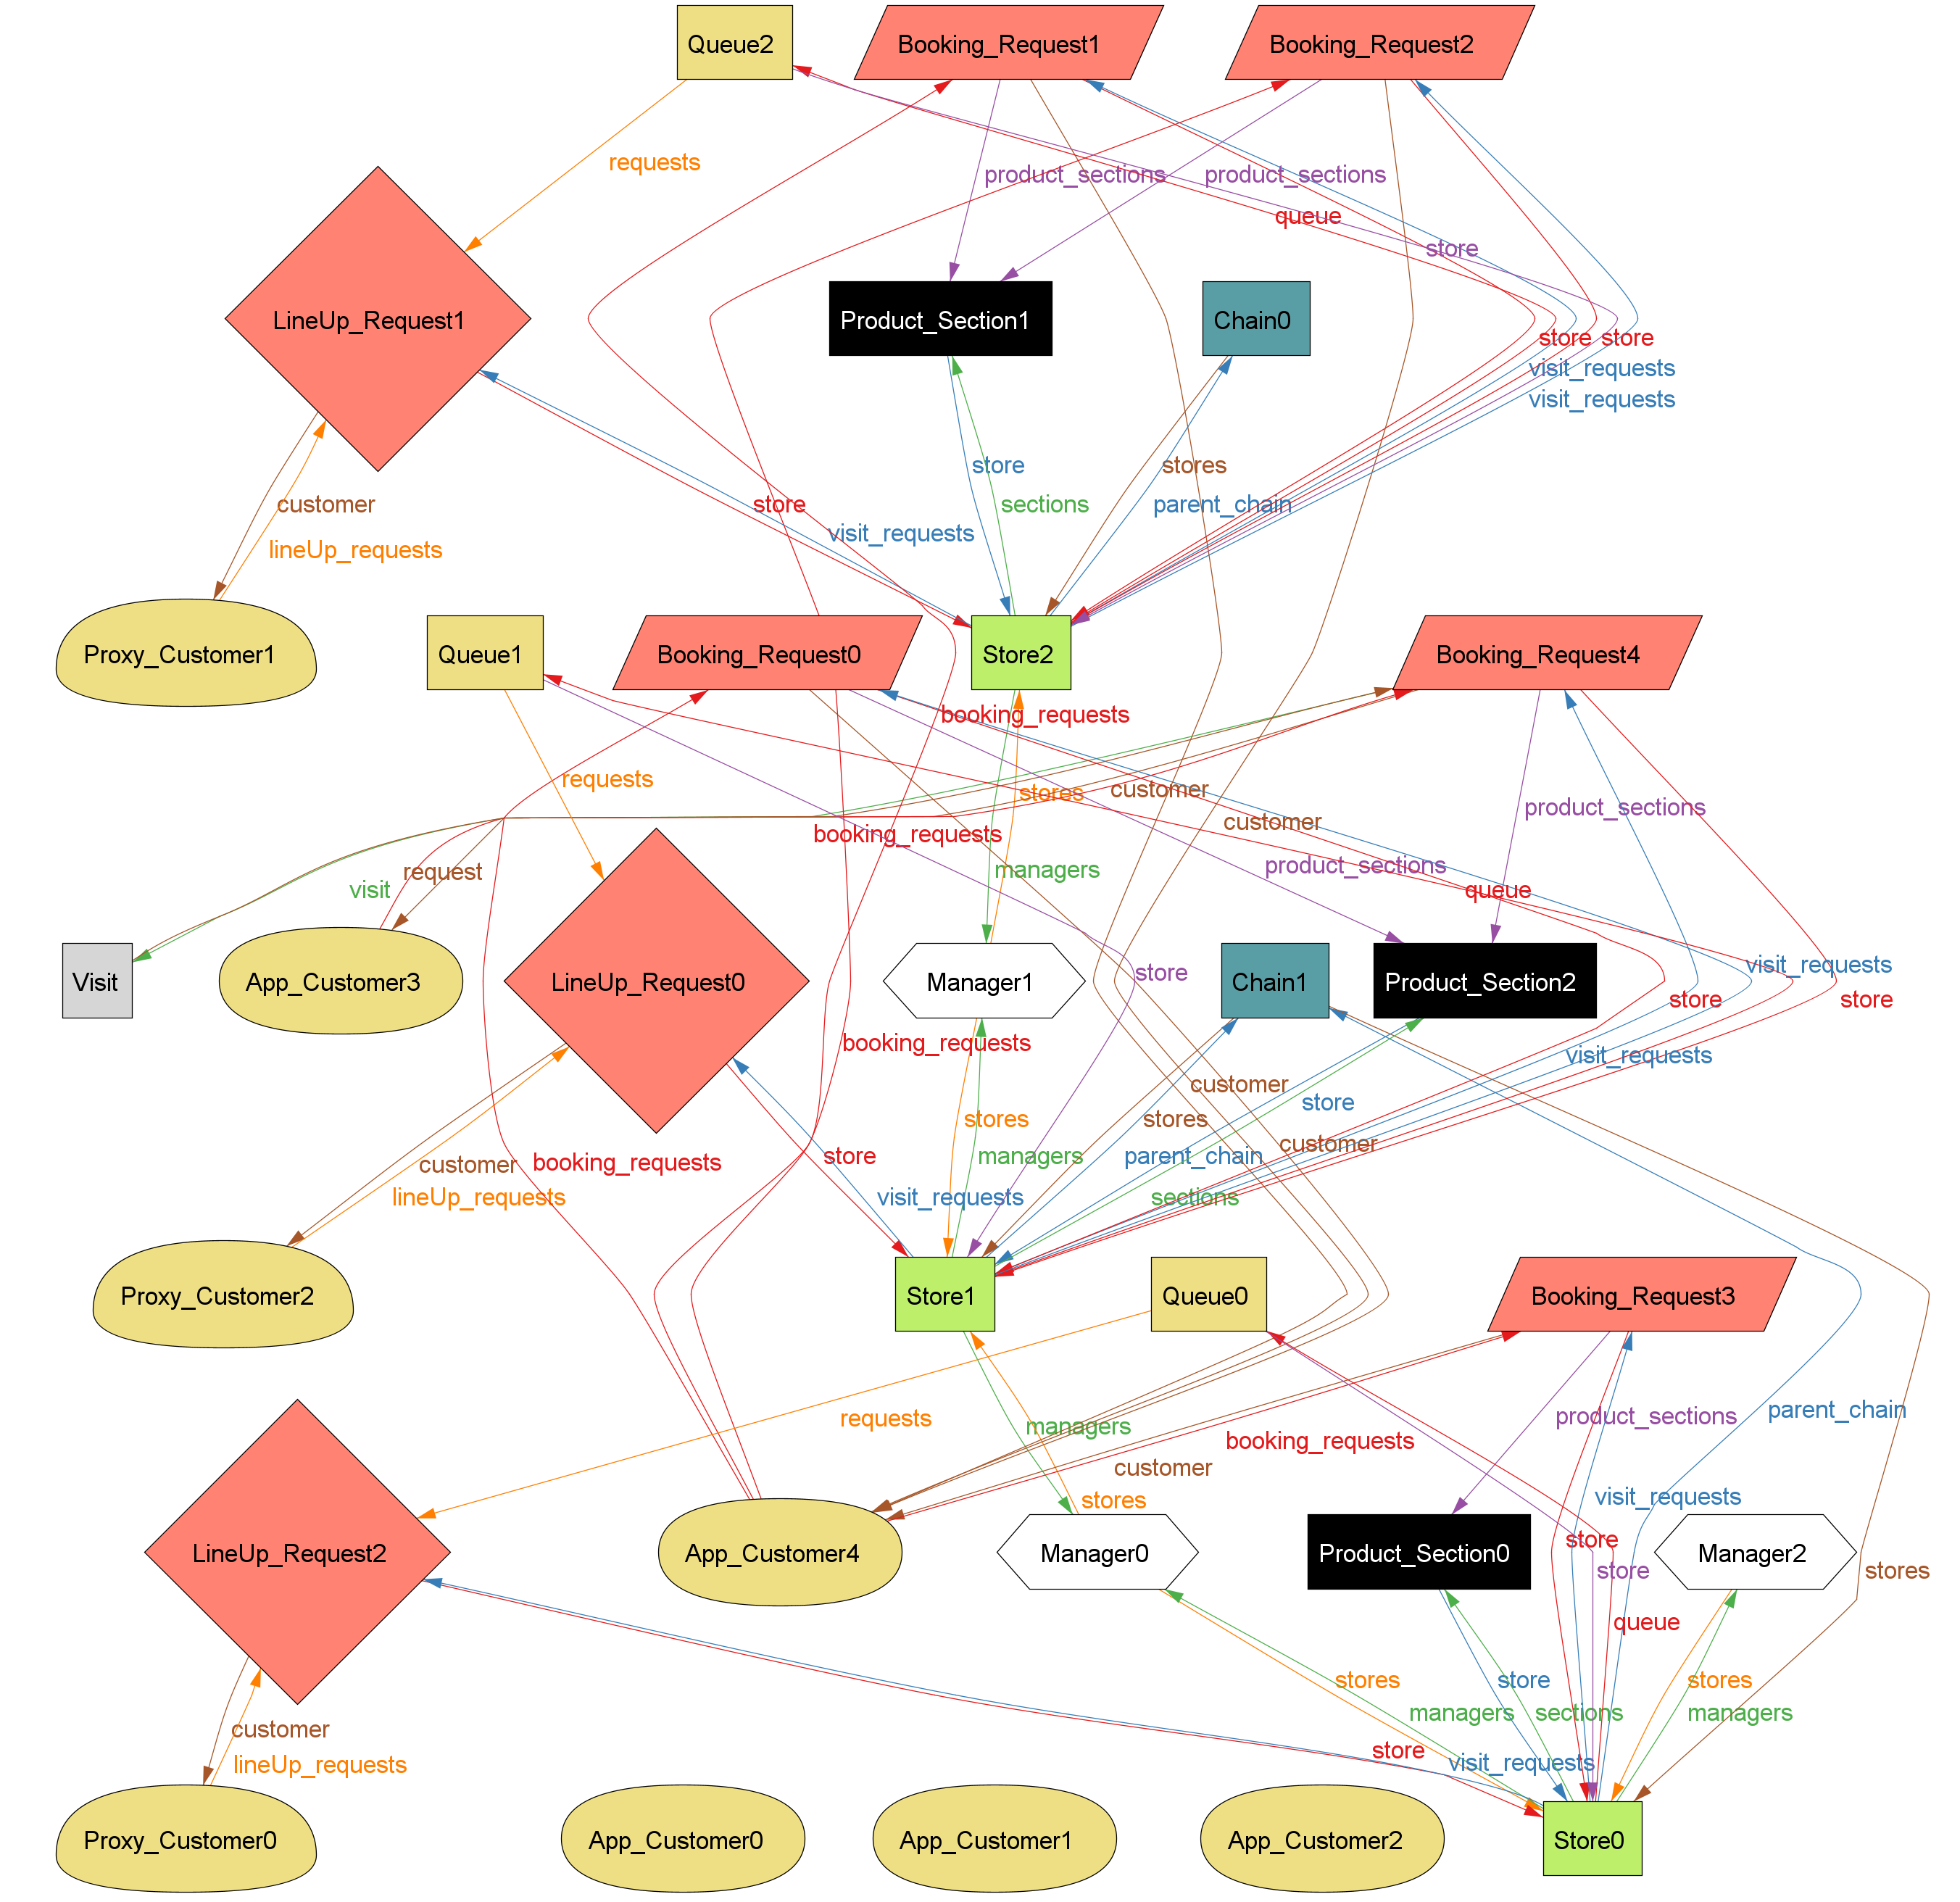
\includegraphics[width=0.9\textwidth, keepaspectratio]{pictures/alloy_instance_diagram}
        \caption{Instance of the alloy model}
        \label{figure:alloy_instance}
    \end{figure}

    
\chapter{Effort spent}
    All the members of the group worked mainly together, in order to guarantee consistency through the entire document. Each member of the group spent approximately 80 hours doing team working. In addition to team working, individual work has been partitioned as shown in the following tables:
    \subsubsection{Riccio Vincenzo}
    \begin{longtable}[c]{|H{.55\textwidth}|c|}
        \hline
        \textbf{Section} & {\bfseries{Hours}} \\ \hline
        \textbf{Team working} & \textbf{80} \\ \hline
        Purpose, goals, scope and phenomena & 2 \\ \hline
        Product perspective & 4 \\ \hline
        Product functions & 1.5 \\ \hline
        Users, assumptions and constraints & 1.5 \\ \hline
        External interfaces & 1.5 \\ \hline
        Functional requirements & 2 \\ \hline
        Use cases & 1.5 \\ \hline
        Sequence and activity diagrams & 1 \\ \hline
        Nonfunctional requirements & 1 \\ \hline
        Alloy & 4 \\ \hline
        Other details of the document & 2 \\ \hline
        \LaTeX & 1.5 \\
        \hline
        \caption{Effort spent -- Riccio Vincenzo}
        \label{table:effort_riccio}
    \end{longtable}
    
    \subsubsection{Sorrentino Giancarlo}
    \begin{longtable}[c]{|H{.55\textwidth}|c|}
        \hline
        \textbf{Section} & {\bfseries{Hours}} \\ \hline
        \textbf{Team working} & \textbf{80} \\ \hline
        Purpose, goals, scope and phenomena & 2 \\ \hline
        Product perspective & 4 \\ \hline
        Product functions & 1.5 \\ \hline
        Users, assumptions and constraints & 2 \\ \hline
        External interfaces & 1.5 \\ \hline
        Functional requirements & 2 \\ \hline
        Use cases & 1 \\ \hline
        Sequence and activity diagrams & 1.5 \\ \hline
        Nonfunctional requirements & 0.5 \\ \hline
        Alloy & 4 \\ \hline
        Other details of the document & 2 \\ \hline
        \LaTeX & 1.5 \\
        \hline
        \caption{Effort spent -- Sorrentino Giancarlo}
        \label{table:effort_sorrentino}
    \end{longtable}
    
    \newpage
    \subsubsection{Triuzzi Emanuele}
    \begin{longtable}[c]{|H{.55\textwidth}|c|}
        \hline
        \textbf{Section} & {\bfseries{Hours}} \\ \hline
        \textbf{Team working} & \textbf{80} \\ \hline
        Purpose, goals, scope and phenomena & 2 \\ \hline
        Product perspective & 3.5 \\ \hline
        Product functions & 1.5 \\ \hline
        Users, assumptions and constraints & 1.5 \\ \hline
        External interfaces & 1.5 \\ \hline
        Functional requirements & 2 \\ \hline
        Use cases & 1 \\ \hline
        Sequence and activity diagrams & 1 \\ \hline
        Nonfunctional requirements & 1 \\ \hline
        Alloy & 3.5 \\ \hline
        Other details of the document & 2 \\ \hline
        \LaTeX & 3 \\
        \hline
        \caption{Effort spent -- Triuzzi Emanuele}
        \label{table:effort_triuzzi}
    \end{longtable}
    
    \chapter{References}
    This chapter contains references to the tools used during the writing of the current document:
    \begin{itemize}
        \item The UML diagram has been designed using the software “StarUML”;
        \item The state charts diagrams, the use case diagram, the sequence diagrams and the activity diagrams have been made using the software “Astah”;
        \item The alloy model has been designed with the official Alloy tool.
    \end{itemize}

\listoftables
\listoffigures

\end{document}